\chapter{Methodology} % Main chapter title
\label{Ch:Method}

\section{The measures of complex networks structure}
%%TODO 2.1 The measures of the complex networks structure

The complex system can be represented by a complex network $G=(V, E)$, where the elements of a system (atoms, proteins, people) map to a set of $N$ nodes $V=\{1, 2, ..., N\}$. The interactions between elements map to $L$ links between nodes, $E = \{ e_1, e_2... e_L\}$. The \textbf{adjacency matrix} ${A} = N \times N$ has value $1$ if there is a connection between two nodes; otherwise, it is $0$ \cite{boccaletti2006complex}.
%TODO Ovakvom recenicnom kao da kazemo da samo imamo binarne mreze. Mozda bi bilo bolje da pre toga kazemo da cemo mi koristiti mahom binarne mreze. I onda ova recenica.
There are a lot of measures to quantify the structure of the network. This section lists the most important measures, such as degree distribution, correlations, and shortest path measures. We also discuss different structures found in the network, such as core-periphery or community structures.  

\subsection{Degree distribution}

The simplest network measure is \textbf{node degree}, $k$. The degree of node $i$ is %gives %TODO is or equal 
the number of nodes adjacent %attached %TODO adjacent
 to node $i$, $k_i = \sum_j A_{ij}$. The network density is the average degree divided by $N-1$, where $N$ is the number of nodes. %It is a relative fraction of nodes in the network.%TODO sta je ovo
 
In the case of regular networks, such as grids, each node has an equal degree, meaning that nodes in the network have similar roles. In the general case, the networks have a more complex structure. If the degree sequence is skewed, we can identify nodes with high-degree (hubs). Removing hubs may partition a connected network into several components \cite{albert2000error}. %%TODO nedostaje citat
 
The degree distribution is the probability that a randomly chosen node has degree $k$. To estimate the degree distribution, we can consider the fraction of $k$ degree nodes $N_k$, $p(k) = N_k/N$. Similarly, we can order nodes according to their degree and plot the node degree.

%To estimate %calculate %TODO estimate. 
%%TODO Bolje bi bilo da uvedes pro sta je P(k) pa onda kako je procenjujemo. 
%the degree distribution, we can consider the fraction of $k$ degree nodes $N_k$, $p(k) = N_k/N$. It is the probability, $P(k)$, that a randomly chosen node has degree $k$. Similarly, we can order nodes according to their degree and plot the node degree.

%If the graph nodes are statistically independent, the degree distribution completely determines the properties of a network \cite{dorogovtsev2002evolution}.%TODO ovo je nejasna recenica
Here we summarize the forms of degree distributions that are mostly found in the complex network theory:
\begin{itemize}
	\item The Poisson distribution. The degree distribution in a random network, where all nodes have the same connecting probability, follows Poisson distribution $P(k)= \frac{(Np)^ke^{-Np}}{k!}$, where $k$ is the mean degree distribution. 
	
	\item Exponential distribution. $P(k) = e^{-k/ \- k}$. It is the degree distribution of the growing random graph. Even for infinite networks, all moments of distributions are finite and have a natural scale of the order of average degree.
	
	\item In many real networks, degree distribution follows a power law. $P(k) = k ^ {-\gamma} $, where $\gamma$ is exponent of the distribution. No natural scale exists in this distribution, so they are called scale-free networks. In infinite networks, all higher moments diverge. If the average degree of scale-free networks is finite, then the $\gamma$ exponent should be $\gamma>2$. Therefore, real networks have a scale-free structure with the emergence of the hubs \cite{newman2010}. 
	%In finite-size networks, fat-tailed degree distributions have natural cutoffs. 
\end{itemize}

When plotting the degree distribution, it is common to use scaling of the axis. As many nodes have a low degree, like for power-law or exponential distribution, it is more useful to use a logarithmic scale. Now it is easier to notice that data points follow a straight line, meaning that degree distribution is some exponential function. 

\subsection{Degree-degree correlations} %%TODO Degree-degree correlations.

Correlation is defined through a correlation coefficient r. If x and y are two stochastic variables, for which we have a series of observation pairs $(x_1, y_1), (x_2, y_2), ...,(x_n, y_n)$. The correlation coefficient $r(x, y)$ between $x$ and $y$ is defined as \cite{van2010graph}:

\begin{equation}
r(x, y) = \frac{\frac{1}{n}\sum_{i=1}^{n}((x_i - \bar{x} ) (y_i - \bar{y}) )}{\sqrt{\frac{1}{n}\sum_{i=1}^{n}(x_i - \bar{x})^2} \sqrt{\frac{1}{n}\sum_{i=1}^{n}(y_i - \bar{y})^2} }
\end{equation}

where $\bar{x} = \frac{1}{n}\sum_{i=1}^{n}x_i$, is the average over variable $x$.

Using the correlation coefficient definition, we can define correlations for vertex degrees. For simple graph G with vertex set $V(G) = \{v_1, ..v_n\}$, $\boldsymbol{A}[i,j] = 1$ if there is a link between nodes $v_i$ and $v_j$. If G is a simple graph with adjacency matrix $\boldsymbol{A}$ and degree sequence $\boldsymbol{d} = [d_1, ..., d_n]$

\begin{equation}
r_{deg}(G) = \frac{\sum_{i=1}^{n}\sum_{i=1+1}^{n}((d_i - \bar{d}) (d_i - \bar{d}) \boldsymbol{A}[i,j] )}{\sum_{i=1}^{n}(d_i - \bar{d})^2}
\end{equation}

An adjacency matrix allows us to calculate the correlations between neighbouring nodes. If two nodes are not connected $A[i,j]=0$, the degree of correlation between them does not contribute to the $r$.

The \textbf{degree-degree correlations} in the network are measured by \textbf{assortativity index}. %%TODO assortativity index ne assortatiity. I nije jedino meren tako,
If correlations are positive, networks are assortative; there is a tendency for connections to existing between similar degree nodes. The negative correlations indicate that large-degree nodes prefer to connect nodes with a small degree, disassortative networks. The average first neighbor degree $k_{nn}$ can be calculated as $k_{nn} = \sum_{k^{'}}k^{'}P(k^{'}|{k})$. The $P$ is the conditional probability that an edge of degree $k$ points to a node with degree $k$. The norm is $\sum_{k^{'}}P(k^{'}|k)=1$, and detailed balance conditions \cite{boccaletti2006complex},  $kP(k^{'}|k)P(k) = k^{'}P(k|k^{'})P(k^{'})$ \cite{boccaletti2006complex}. If the node degrees are uncorrelated, $k_{nn}$ does not depend on the degree; otherwise, increasing/decreasing function indicates positive/negative correlations in the network \cite{park2003}.

The Newman defined the assortativity \cite{newman2002assortative} index $r$ in slightly different way:

\begin{equation}
r = \sum_{kl}kl(e_{kl} - q_lq_k) / \sigma_q^2 ,
\end{equation}

where $e_{kl}$ is the probability that a randomly selected link connects nodes with degrees $k$ and $l$, $q_k$ is a probability that a randomly chosen node is connected to node $k$ and equals $q_k = kp_k / \langle k \rangle$, while $\sigma_q$ is a variance of the distribution $q_k$. 

\subsection{Clustering coefficient}

The \textbf{clustering coefficient} is a measure describing the neighbourhood's structure. In networks, exist a tendency to form triangles or clusters \cite{barabasi2016network}. It is common in friendship networks where two friends of one person have a high probability of being friends. %TODO citat nedostaje
The clustering can be measured by computing the number of links between neighbours of one node,
\begin{equation}
c_i=2e_i/(k_i(k_i-1))
\end{equation}

We can calculate the mean clustering coefficient by averaging it overall network nodes. It ranges from  $\langle c \rangle = 0$ where connections between neighbouring nodes do not exist; the network has a tree structure. On the other hand, $\langle c \rangle = 1$ indicates a fully connected network. 

Newman proposed the alternative definition for the clustering coefficient based on the number of triples and triangles in a graph \cite{newman2009random}. A triangle at node $v$ is a complete subgraph with three nodes, including $v$. A triple on the node v is a subgraph of exactly three nodes and two edges, where v is incident with two edges. The network transitivity is the ratio of the number of triangles in the network over the number of triples. The network transitivity is seen as global clustering, as it considers the whole network.  

\subsection{Paths} %Network paths} %TODO moze samo paths
In the network structure, the interacting nodes are directly connected with the edge. In this representation, the distance between them is $d_{v_i, v_j} =1 $. Distance defined like this does not have any physical meaning, and its purpose is to describe how the position of nodes in the network structure influences the other distant nodes. 

The \textbf{path} between two nodes \cite{van2010graph}, $v_i$ and $v_j$ is a sequence of edges $\{(v_1, v_2),  (v_2, v_3), ...(v_k, v_{k+1})\\,... (v_{n-1}, v_n)\}$, where $v_1=v_i$, $v_n=v_j$. In the path, the nodes are distinct. Otherwise, the sequence is called a \textbf{walk}, where each node can be visited many times. Also, it is possible to define a \textbf{cycle}, a path that starts and ends on the same node while other nodes in the cycle are distinct. The length of the path, walk or cycle is the number of links in the sequence. We can easily calculate the number of walks between two nodes using the adjacency matrix. The $A^2$ gives us walks of length $2$, the $A^3$, the number of walks of length 3, and so on. 

The network is connected if it can define the path between every two nodes. When it is not the case, the network is disconnected into two or more connected components. Note that the component can be an isolated node. Also, in directed networks may happen that node $v_i$ is reachable from node $v_j$, but if we start from $v_j$, we can not find the path to the $v_i$. Such a graph is connected but is called a weakly connected component \cite{jackson2010social}.

We can find different paths between two nodes in the network, but the most important one is the \textbf{shortest path} \cite{van2010graph, jackson2010social}. The distance between two nodes $d(v_i, v_j)$ is defined as the shortest path length between two nodes. 
In the case of weighted networks, it is the path with minimal weight, and the length of such a path does not have to be minimal. Distances on the network can give us insight into how similar networks are and indicate the node's relative importance in the network. 

%The node's eccentricity shows how far the farthest vertex is positioned in the network. 
The \textbf{radius} is the minimum overall eccentricity value. In contrast, the \textbf{diameter} defines the largest distance between nodes in the network \cite{van2010graph}. These definitions apply to directed and undirected graphs. 

If G is a connected graph with vertex set V and $\bar{d}(u)$ is the average length of the shortest paths from node u to any other node v in network G \cite{van2010graph}.

\begin{equation}
\bar{d}(u) = \frac{1}{|V|-1} \sum_{v\in V, v \notin u} d(u,v)  
\end{equation}

From there, the \textbf{average path length} is the mean value over $\bar{d}(u)$.

\begin{equation}
\bar{d}(G) = \frac{1}{|V|}\sum_{u \in V} \bar{d}(u)
\end{equation}

while the \textbf{characteristic path} length of G is median over all $\bar{d}(u)$.


\subsection{D-measure}

For each node $i$, we can define the distribution of the shortest paths between node $i$ and all other nodes in the network, $P_{i}=\{p_{i}(j)\}$, where $p_{i}(j)$ is percent of nodes at a distance $j$ from node $i$. The connectivity patterns can efficiently describe the difference between the two networks.    
To specify how much $G$ and $G^{'}$ are similar we use D-measure \cite{tiago2}
\begin{equation}
D(G, G^{'}) = \omega \left| \sqrt{\frac{J(P_1,..P_N)}{log(d)}}-\sqrt{\frac{J(P_1^{'},..P_N^{'})}{log(d^{'})}} \right| + (1-\omega) \sqrt{\frac{J(\mu_{G},\mu_{G^{'}})}{log2}}
\label{eq:dmeasure}
\end{equation}

D-measure calculates Jensen-Shannon divergence between $N$ shortest path distributions,

\begin{equation}
J(P_1,.., P_N)) = \sum_{i,j}p_i(j)log(\frac{p_i(j)}{\mu_j})
\end{equation}

where  $\mu_j = (\sum_{i=1}^N p_i(j))/N$ is mean shortest path distribution.

The first term in equation \ref{eq:dmeasure} compares local differences between two networks, and Jensen-Shannon divergence between $N$ shortest path distributions $J(P_{1},..., P_{N})$ is normed with network diameter $d(G)$. The second part determines global differences, computing  ${J(\mu_{G},\mu_{G^{'}})}$ between mean shortest path distributions. The D-measure ranges from $0$ to $1$. The lower D-measure is, the more similar networks are, and structures are isomorphic for D-measure $D = 0$.

\newpage
\section{Community structure}

Nodes can be organized into groups called communities. In social networks, communities indicate that people share some common interests, or in biological networks, we can find that genes or neurons with similar functions are grouped. Identifying these hidden blocks can lead to interesting insights into the network. However, the community detection problem does not give a precise characterization of what a community is. A standard definition of a community is densely connected subgraph \cite{fortunato2010community, martin}, meaning that nodes in one community tend to associate, creating the assortative connectivity pattern. On the contrary, nodes could be organized in disassortative communities, where connections between groups are denser. 

The network with $k$ communities could be represented using $k \times k$ matrix $p$. The diagonal elements of $p$ indicate the density inside communities, while off-diagonal elements show the density between groups. Figure \ref{fig:SBM} \cite{fortunato2010community} shows the matrix and networks for two communities. In the first example, (\ref{fig:SBM} a), the diagonal elements have a higher probability, as in the classic definition of assortative community structure. In disassortative structure (\ref{fig:SBM} b), more connections exist between two partitions than inside them, i.e. off-diagonal elements have higher probabilities. Bipartite networks can be represented as a disassortative network with two groups. The links exist only between communities. Figure (\ref{fig:SBM} c) shows the core-periphery network. This network structure is composed of a core where nodes are well connected with itself and with the periphery. The connectivity inside the periphery is sparse. Finally, if there is no difference between connectivity inside and between groups, the concept of communities is lost. We can treat the whole network as a single community, where each node has the same connectivity probability, i.e. as Erdos Renyi random graph. 

\begin{figure}[h]
	\centering
	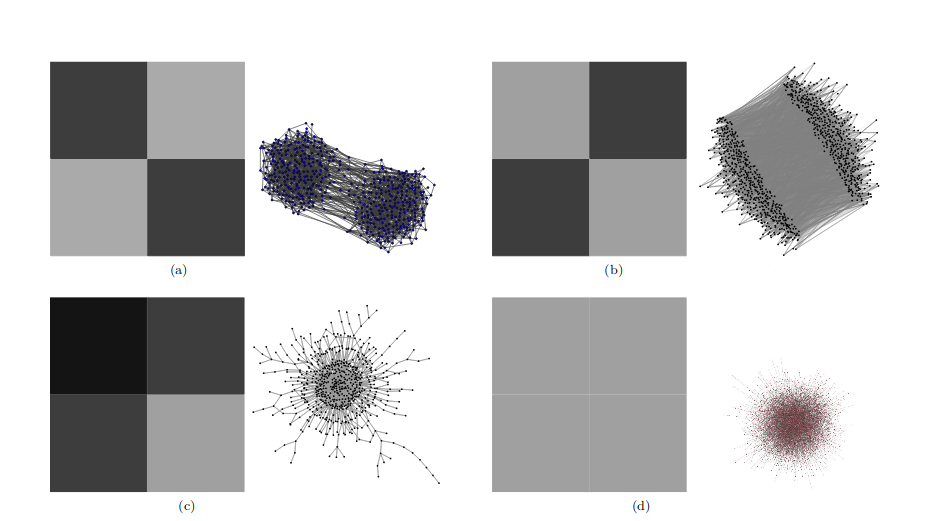
\includegraphics[width=0.8\textwidth]{chapter2/structures.png}
	\caption[Stochastic Block Model]{ Different communities structures  (a) assortative. (b) disassortative. (c) core-periphery. (d) Erdos Renyi random graph.}
	\label{fig:SBM}
	%TODO ima li ova slika u boji?
\end{figure}

Different algorithms are used for detecting the community structure in the underlying network, optimizing different objective functions of the network partition. Still, if the ground-truth communities are unknown, there are no guarantees that we will infer the actual number of communities and entirely correct node assignments. Even though community detection algorithms are widely used in complex network analysis as they can give us a better understanding of network structure. %TODO citat
In this section are explained two community detection models, the first one based on optimizing the modularity function, and the other based on the statistical inference of the Stochastic Block Model (SBM) where is optimized the likelihood function. %TODO citat

\subsection{Louvain algorithm}

Comparing the link density of the community with the link density obtained for the same group of nodes randomly connected, we could conclude if the community corresponds to the dense subgraph or if the structure is created entirely random. The \textbf{modularity} \cite{guimera2004modularity, good2010performance} is a function that measures the randomness of each partition. %TODO definisati sta je partition
We can compare the communities with modularity and decide which one is better. For the network with $N$ nodes and $L$ links that partitions into $n_c$ communities. Each community has $N_c$ nodes and $L_c$ links. If the number of connections is larger than the expected number of links between $N_c$ nodes given in the expected node sequence, these nodes may form the community. We calculate the difference between real network connectivity $A_{ij}$ and the expected number of links between nodes if the network is randomly connected, $p_{ij}$. The $p_{ij}$ can be obtained by randomizing the original network but keeping the expected degree of each node unchanged, so $p_{ij}= \frac{k_ik_j}{2L}$.

\begin{equation}
M_c = \frac{1}{2L}\sum(A_{ij}-p_{ij})
\end{equation}

If modularity is positive, the selected nodes may be a community, as their connectivity is far from random. If $M_c$ is zero, then the connectivity between nodes is arbitrary, and if $M_c$ is negative, the nodes do not form the community. 

The same idea can be generalized to the whole network: The modularity of the network partitioned into $n_c$ communities is then defined as:
\begin{equation}
M=\sum_{c=1}^{n} [\frac{L_c}{L} - (\frac{k_c}{2L})^2]
\end{equation}

The higher modularity indicates that nodes are partitioned in better communities. When we put all nodes into only one community $M=0$, otherwise, if each node is the community itself $L_c=0$ and the sum is negative. Maximum network modularity indicates the best partions. As too many possible partitions exist, we need an algorithmic approach to identify the best separation. 

The first algorithm proposed for modularity optimization was \textbf{greedy algorithm}. First, it assigns each node to a community and starts with N communities. Then, we should merge each pair of communities and calculate the modularity difference $\Delta M$. We can join those two communities by identifying the pair for which the difference is the largest. It is repeated until all nodes merge into a single community. The best partition is one with the largest $M$. 

\textbf{Louvain algorithm} \cite{blondel2008fast} is an optimization algorithm with better scalability than the greedy algorithm so it can operate on very large networks. Initially, each node is assigned to a different community, and similar to before, we calculate the difference in the modularity moving nodes to one of their neighbouring community. Then we move node $i$ to the community such that modularity becomes larger. It is applied to all nodes until no further improvement can be made. In the second step, we create a weighted network whose nodes are communities identified during the first step. The weight of the links between communities is the sum of the weights between nodes. The number of links inside the community is given as a weighted self-loop. Then, the first and second spets are repeated until there is no more change in the modularity. %TODO Posto je sekcija o Louain algoritmu, treba dodati jos par paragrafa o njemu. Konkretno njegove karakteristike (otezinjeni, usmereni grafovi...), zatim reyolucija, i najbitnije kako odredjuje optimalan broj zajednica. Pogledaj neki od Santoih poslednjih radoa na temu zajednica.

\subsection{Stochastic block model}

Another approach for studying the community structure of complex networks, the Stochastic Block Model (SBM), assumes that nodes are clustered in the groups, and the relations between nodes depend on the probabilities for group memberships \cite{lee2019review}. In one group, nodes have similar connectivity patterns. To describe the network G with the SBM model, we need to define the following:

\begin{itemize}
	\item k: number of groups
	\item group assignment vector, g: $g_i \in\{1,2..k\}$, gives the group index of node $i$.
	\item SBM matrix, $p_{k \times k}$, whose elements $p_{rs}$ are the probabilities that edges between groups $r$ and $s$ exist. Note that nodes within one group have the same connection probabilities. 
\end{itemize}

The number of possible nodes between two groups $r$ and $s$:
\begin{equation}
n_{rs} = \begin{cases}
n_r(n_{r}+1)/2 &\text{if  } r=s \\
n_rn_s &\text{if  } r=s\\, 
\end{cases}
\end{equation}
while the number of possible edges depends on the adjacency matrix $A_{ij}$:
\begin{equation}
e_{rs}=\frac{1}{1+\delta_{rs}}\sum_{i \in r, j\in s} A_{ij}
\end{equation}



The benefit of this model is that we can \textbf{generate} many networks with similar network structure \cite{rosvall2019different}. When model parameters are initialized, the network can be easily generated. For each pair of nodes $i$ and $j$ in network $G$, we draw a link if random number $r_{ij}<p_{r, s}$. 

The likelihood of generating network $G$ for given model parameters is:
\begin{equation}
P(G|p, g) = \prod_{i,j} Pr(i \rightarrow j| p, g) = \prod_{(i,j)\in E} Pr(i \rightarrow j| p, g)\prod_{(i,j)\notin E} ( 1 - Pr(i \rightarrow j| p, g))
\end{equation}

In the processes where the connection between two nodes is described with Bernoulli distribution, the likelihood takes the form:
\begin{equation}
P(G|p, g) = \prod_{(i,j)\in E} p_{g_ig_j}\prod_{(i,j)\notin E} ( 1 - p_{g_ig_j})
\end{equation}

In the likelihood equation, we iterate over all pairs of nodes, separating the product over edges present in the network and edges that are not present.  
As all nodes are considered independent, we can switch the product over nodes with the product over groups such that
\begin{equation}
P(G|p, g) = \prod_{(r,s)} p_{rs}^{e_{rs}}(1-p_{rs})^{n_{rs}-e_{rs}}
\end{equation}
As it is easier to work with the logarithm of the likelihood function, after taking the logarithm of the likelihood function, we get the following expression:
\begin{equation}
L = log(P(G|g, p)) = \sum_{r,s} e_{r,s} ln\frac{e_{rs}}{n_{rs}} + (n_{rs}-e_{rs})ln(\frac{e_{rs}-e_{rs}}{n_{rs}})
\end{equation}

Instead of generating networks, the opposite task is network \textbf{inference}. For a given network $G$, and specified the number of communities $k$, we can use the SBM model to infer the nodes' assignments into groups, so we need to choose vector $g$ and SBM matrix $p$ such that the likelihood for generating network $G$ is maximized. 

The formulation of the SBM model does not consider how to infer the optimal number of groups. Optimizing the likelihood function for different numbers of groups would increase likelihood while each node is not assigned to a different group. In practice, our found community structures for a fixed number of groups, and then the likelihood function could be penalized by the number of model parameters. One approach is calculating the \textbf{Minimum description length (MDL)}. For the variable that occurs with probability P(x), the necessary amount of information to describe it is $-log_2P(x)$. The numerator of posterior probability could be written as
\begin{equation}
P(G|g)P(g) = P(G|p, g)P(p, g)=2^{-\Sigma}
\end{equation}
where $\Sigma$ is the data's description length (DL). It means that if we find the network partition that maximizes the posterior distribution, we also find the MDL. The MDL consists of two terms: $\Sigma = -log2(p(G|p,g))-log2P(p,g)$. In the first part of the equation, the amount of information necessary to describe the model decrease with the number of groups. The second contribution comes only from the model, and as the model becomes more complex, with a larger number of groups, this part increases. The optimal solution represents the balance between these two terms in the MDL equation.  

This SBM model has many variants motivated by specific properties of real data. For example, for degree heterogeneous networks, there is degree corrected SBM \cite{karrer2011stochastic}. In some social networks, users can belong to more than one group, which can be modelled with mixed membership SBM. Other extensions include application to bipartite, weighted network, and hierarchical model \cite{funke2019}. Many community detection algorithms define the community as an assortative structure. With the SBM model, such limitations do not exist, and it is possible to directly use statistical inference for discovering core-periphery structures or even networks with bipartite structures.  

\subsection{Core-periphery structure}


Core-periphery structure describes a network whose nodes are divided into two communities, densely connected core and less connected periphery \cite{csermely2013structure}. With the average probabilities of edges within each group as $p_{11}$ and $p_{22}$, and between groups $p_{12}$, the core-periphery structure is defined under the condition  $p_{11}> p_{12} > p_{22}$. The simple method for finding core-periphery structures assumes that core nodes have higher degrees in the core than in the periphery. Another simple method is to construct k-cores \cite{malliaros2020core}. K core is a group of nodes connected to at least k other members. K-cores form a nested set and become denser with higher k. The core-periphery structure can be detected by optimizing the measure similar to modularity, as defined by Borgatti and Everett \cite{borgatti2000models}. Their goal is to find the division that minimizes the number of edges in the periphery. So they define the score function as equal to the number of edges in the periphery minus the expected number of such edges placed randomly. $\rho = \frac{1}{2}\sum_{ij}(A_{ij}-p)g_ig_j$.

Another way to detect core-periphery structure is to use the inference method based on fits to a Stochastic Block Model (SBM) \cite{zhang2015identification, karrer2011stochastic}. In this method, we fit the observed network to a block model with two groups, such that edge probabilities have the form $p_{11}> p_{12} > p_{22}$. Vector $\theta_i = r$ indicates that node $i$ is in block $r$, while SBM matrix $\{p\}_{2x2}$, specify the probability $p_{rs}$ that nodes from group $r$ are connected to nodes in group $s$. The SBM model is looking for the most probable model that can reproduce a given network G \cite{gallagher2020clarified}. 
Probability of having model parameters $\theta, p$ given network $G$ is proportional to the likelihood of generating network $G$, prior of SBM matrix $P(p)$ and prior on block assignments $P(\theta)$: $P(\theta, p| G) = P(G | \theta , p) P(p) P(\theta)$, while the likelihood function takes following form: $P(G | \theta , p) = \prod_{i<j} p_{r_is_j}^{A_{ij}}(1-p_{r_is_j})^{1-A_{ij}}$, where $A_{ij}$ is a number of edges between nodes $i$ and $j$. The prior $P(p)$ is modified for core-periphery model such that $P(p)  \sim I_{0<p_{22}<p_{12}<p_{11}<1}$, while prior  $P(\theta) $ consists of three parts: probability of having $2$ blocks; given the number of layers probability $P(n|2)$ of having groups of sizes ${n_1, n_2}$ and the probability $P(\theta|n)$ of having particular assignments of nodes to blocks. 


\newpage
\section{Network models}
%TODO Ovde treba ubaciti samo jedan pasus zasto su nam bitni modeli. Cemu sluze, zasto ih pravimo i slicno.

\subsection{Random network model}

The random graph model was introduced by mathematicians Paul Erdős and Alfred R\' {e}nyi in 1959. In this model, connections between nodes are chosen randomly, and every link has the same probability of existing. The graph is characterized only by a number of the nodes $N$ and the linking probability $p$, so Erdős-R\' {e}nyi graph is written as $G(n, p)$. 

The creation of ER random network consists of the following steps:
\begin{itemize}
	\item we start with $N$ isolated nodes
	\item between each $N(N-1)/2$ pair of nodes we create link with probability $p$; sampling random number $r \in (0,1)$, we create link if $r \leq p$    
\end{itemize}


\begin{figure}[H]
	\centering
	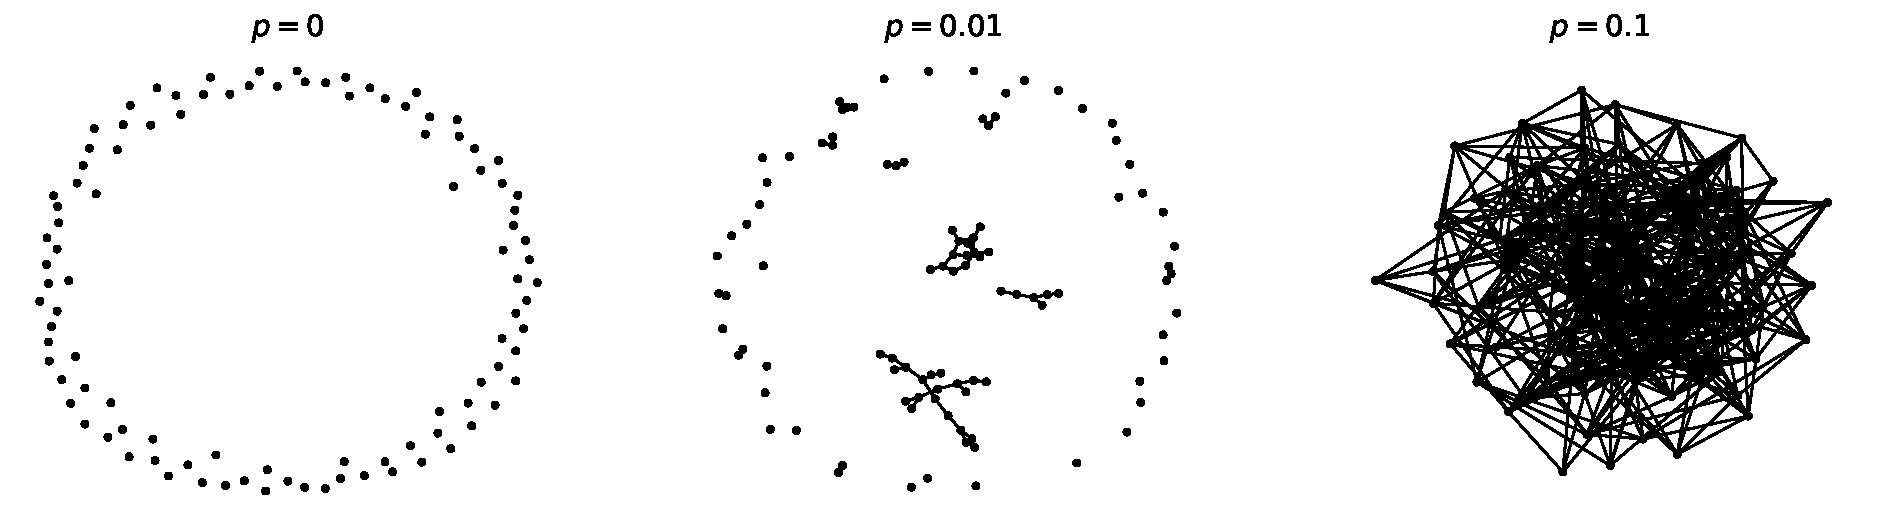
\includegraphics[width=0.9\linewidth]{chapter2/ERgraph.pdf}
	\caption[Erdős-R\' {e}nyi]{Erdős-R\' {e}nyi graph with $N=100$ nodes and different linking probabilities $p$.}
	\label{fig:erp}
\end{figure}

We should note that this process is stochastic. The networks $G(N, p)$ with the same parameters do not need to have the same structure; i.e. they differ in the number of links. Therefore, the single random graph is only one of all the possible realizations in the statistical ensemble. 

Two simple quantities that could be estimated are the average number of links and the average degree. For a complete graph with $N$ nodes, the number of edges is $N(N-1)/2$. As the probability of drawing every edge is $p$, the \textbf{average number of links} is given as 

\begin{equation}
\langle L \rangle = \frac{N(N-1)}{2}p
\end{equation}

We conclude that the network's density equals probability $p$.
The \textbf{average degree} is approximated as $\langle k \rangle = 2 \langle L \rangle / N $, leading to:

\begin{equation}
\langle k \rangle = (N-1)p 
\end{equation}

The \textbf{degree distribution} of ER random graph follows the binomial distribution \cite{barabasi2016network}. 

\begin{equation}
P(k) = \binom{N-1}{k}p^k(1-p)^{N-1-k}
\end{equation}

The probability that the node has degree $k$ is given with the second term $p^k$, while the probability that other N-1-k links are not created is given with the third part of the equation. Finally, there are  $\binom{N-1}{k}$ combinations for one node to have $k$ links from $N-1$ possible links. 

The binomial distribution describes very well small networks, see Figure \ref{fig:erdist}. For larger networks, we find that they are sparse and that the average degree is much smaller than a number of nodes $\langle k \rangle << N$. In this limit, binomial distribution becomes the Poisson, as could be shown on Figure \ref{fig:erdist} which now depends only on one parameter $\langle k \rangle$

%%TODO pozvati se na sliku
%TODO ispraviti naziv na slici

\begin{equation}
p(k) = \frac{1}{k!}e^{-\langle k \rangle}\langle k \rangle^{k}.
\end{equation}

\begin{figure}[H]
	\centering
	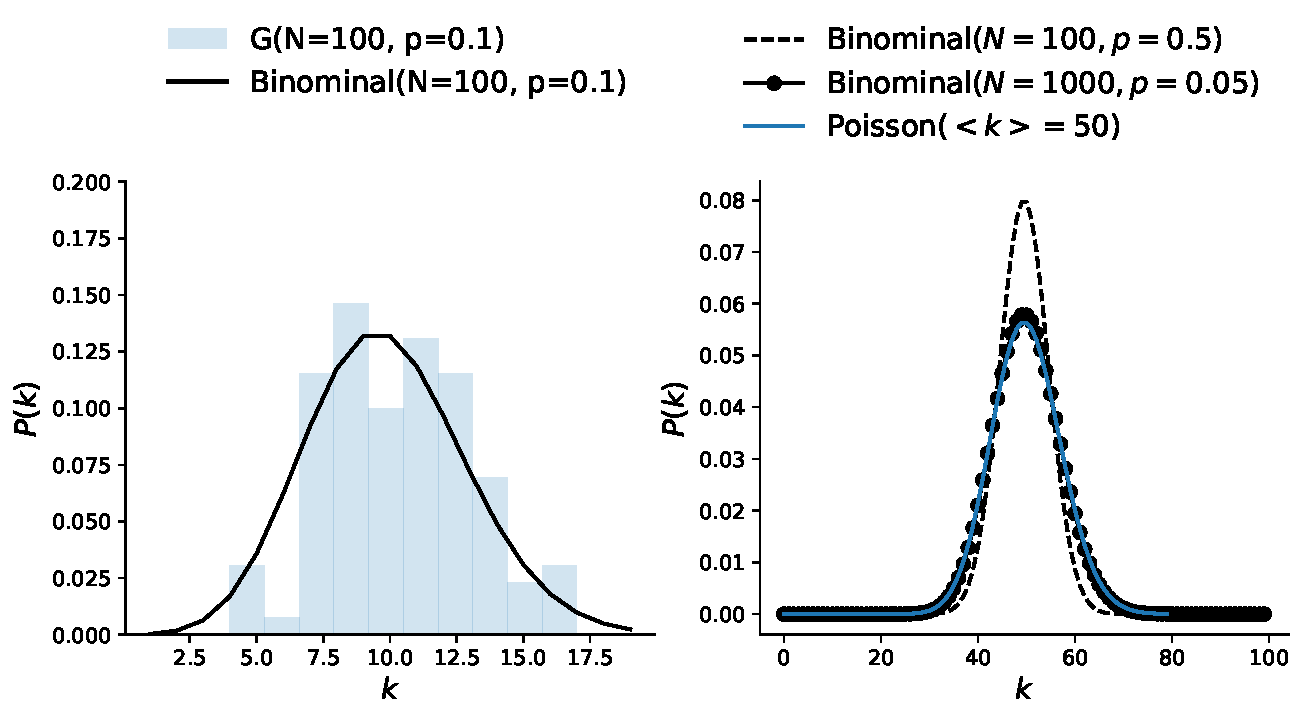
\includegraphics[width=0.9\linewidth]{chapter2/ER_dist.pdf}
	\caption[Degree distribution of Erdős-R\' {e}nyi graph.]{Degree distribution of ER graph. The degree distribution of small networks follows binomial. Larger networks are better approximated with Poison distribution, and degree distribution for fixed average degree $<k>$ becomes independent of the network size.}
	\label{fig:erdist}
\end{figure}

The random graph has a very small \textbf{average path length}, it is given as $\langle l \rangle = \frac{ln N}{ln(pN)}$ that is characteristic of many large networks \cite{bollobas2003mathematical}. The clustering coefficient is proportional to linking probability, $\langle C \rangle = p$, so we find a small clustering coefficient in large random networks, contrary to real-world networks.  %about small networks Barabasi chapter3, page 22

Figure \ref{fig:erp} shows how the network becomes more connected by increasing the linking probability $p$. When $p=0$, all nodes are disconnected. In the other limit, $p=1$, the network is fully connected. Between those two probabilities exists critical probability, where the giant component appears. The giant component is a sub-graph whose size is proportional to the network size. In other words, the network does not have disconnected components. Such change in the network is a phase transition in network connectivity and is related to percolation theory. 

The phase transition occurs when the average degree is $ \langle k  \rangle = 1$, which gives us: $p_c = \frac{1}{N-1}$, meaning that all nodes have degree larger than one \cite{barabasi2016network}. When the $ \langle k  \rangle < 1$, the network is in the sub-critical regime where all components are small. In the critical regime, the size of the giant component is proportional to the $N^{2/3}$. In the supercritical regime, $ \langle k  \rangle > 1$, the probability of a giant component appearing is 1.

\subsection{Small-world networks}

Inspired by the idea that real-world networks are highly clustered, and the average distance is small, Watts and Strogatz \cite{watts1998collective} proposed the "small-world" model. The model starts from the regular lattice, and with rewiring links, the network starts to resemble small-world property. The procedure is the following:

\begin{itemize}
	\item At the beginning, nodes are placed on the ring lattice, see Figure \ref{fig:wsgraph}, and each node is connected to $k/2$ first neighbours on the left and the right side. Initially, the clustering coefficient is high, $c=3/4$. 
	\item For each link in the network, with probability $p$, we choose a random node to rewire the link. This makes long-distance nodes connect, decreasing the network's average path length, Figure \ref{fig:wsgraph}.
\end{itemize}

The model interpolates between the regular graph when the probability is $p=0$ and the random graph with $p=1$ when all links are randomly rewired. Short distances and high clustering are present in the network  for the critical probabilities ranging from $p \approx 0.01 - 0.1$ \cite{watts1998collective}. %%TODO kolika je verovatnoca

\begin{figure}[H]
	\centering
	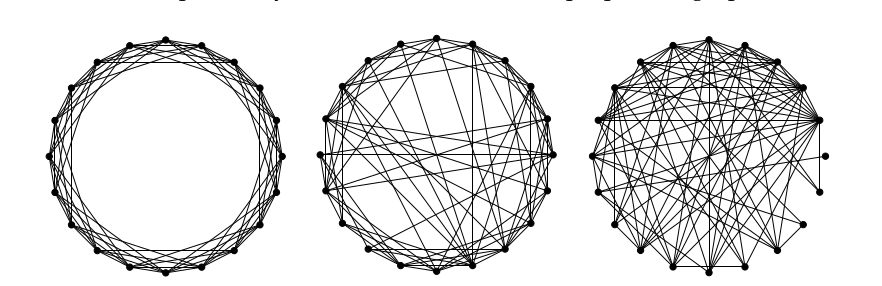
\includegraphics[width=0.9\linewidth]{chapter2/ws_graph.png}
	\caption[Watts and Strogatz graph model creation]{Watts and Strogatz graph model creation.}
	\label{fig:wsgraph}
\end{figure}

Even though the small-world network model lacks the power-law degree distribution found in real-world networks, it is an important model that motivated the research on random graphs. 

\subsection{Barab\' {a}si-Albert model}

The ER random graph model and WS small-world model are static models where the number of nodes is fixed. It is one of the reasons why they can not fully explain the properties of real systems. The size of real systems does not remain constant; real networks grow. Growth means that at each time step, new nodes are added to the network. The simplest model that produces scale-free networks is the Barabasi-Albert model \cite{barabasi1999}.

\begin{itemize}
	\item The model starts from the small number, $n_0$ randomly connected nodes, with $m_0$ links.
	\item At each time step, a new node with $m$ links joins the network. A new node creates links with the nodes already present in the network, following the linking rules; in this case, preferential attachment rules. 
\end{itemize}

The preferential attachment is important for generating a system with scale-free properties. In the real system, the linking between nodes is not a random process; the preference for specific types of nodes exists. For example, popular web pages can quickly get more visits, or it is expected that already popular papers will get more citations. This effect is also called rich-get-richer or preferential attachment.

The simplest formulation of the preferential attachment model is that new nodes tend to connect with high-degree nodes. The linking probability $\Pi$ is then proportional to node degree $k$:  

\begin{equation}
\Pi(k_i) = \frac{k_i}{\sum_jk_j} 
\end{equation} 

As at each step one node arrives, we can estimate the number of nodes at the time step t, $N(t) = n_0+t$, with links $L(t) =m_0+ mt$. 

First, we can calculate the evolution of network degrees in time.
\begin{equation}
\frac{dk_i}{dt} = m\Pi(k_i) = m\frac{k_i}{\sum_jk_j} = m\frac{k_i}{m_0 + 2mt}
\end{equation}

Note that the new node that arrived at time point $t_i$ has degree $m$, as it links to $m$ old nodes. Solving the equation, we get that at $t>t_i$, it has a degree that grows as the square root of time; it also shows that younger nodes easily acquire a larger degree. 
\begin{equation}
k_i(t) = m \left(\frac{t}{t_i}\right)^{\frac{1}{2}}
\end{equation}


Degree distribution follows power-law, and for large k is approximated with $P(k) = k^{-\gamma}$, such that $\gamma=3$. More precisely, the degree distribution has form \cite{krapivsky2010kinetic}:

\begin{equation}
P(k) = \frac{2m(m+1)}{k(k+1)(k+2)}
\end{equation}

For large $k$, it is exactly the power law. It is also independent of the time and size of the system, meaning the emergence of a stationary scale-free state. Distributions do not depend on the N. If we vary $m$, the slope of distributions is the same, but they are parallel. After rescaling $p(k)/m^2$, they fall on the same line \cite{barabasi2016network}.
% TODO Glavna karakteristika BA modela je power-law degree distribution, To ovde nije ni priblizno ocigledno. Bilo bi lepo da postoji i slika., 

%stationary degree distribution does not depend on the system parameters, so different systems have similar behaviour

As the network grows, nodes with larger degrees become bigger, so we end up with few nodes with many links, called hubs. The \textbf{network diameter}, represents the maximum distance in network, $d \sim \frac{lnN}{lnlnN}$ \cite{bollobas2003mathematical}. The diameter grows slower than $lnN$, making the distances in the BA model smaller than in the random graph. The difference is found for large N. It is known that the BA network has hubs that shorten the path between less connected nodes. Also, if hubs are removed from the network, the network easily partitions into several components, losing its properties. The \textbf{clustering coefficient} of the BA model follows $C \sim \frac{ln N^2}{N}$ \cite{bollobas2003mathematical}. It differs from clustering found in random networks, and BA networks are generally more clustered. 

The combination of the growth and preferential attachment linking is crucial for getting scale-free networks \cite{barabasi1999}. For example, eliminating the preferential attachment; in a growing network with random linking, degree distribution is stationary but follows exponential. In contrast, the absence of growth leads to the non-stationary degree distribution. When a number of nodes is fixed, the network grows only in the number of links, such that randomly chosen node $i$ connects to node $j$ according to probability $\Pi$. In the beginning, the degree distribution follows the power law, the same as in the BA model. As more links are added to the network, the distribution changes its shape; first, the peak appears, while at the end network becomes a complete graph, where all nodes have the same degree.  

\subsection{Nonlinear preferential attachment model}

In the nonlinear preferential attachment model linking probability also depends on the node degree. The dependence is not linear and has the following a form \cite{krapivsky2001}:

\begin{equation}
\Pi(k_i) = {k_i}^{\beta}
\end{equation} 

The probability that a newly added node attaches to node $i$ depends on the existing $i$-th node degree $k_i$ and the parameter $\beta$. When $\beta=1$, the model is the BA model, where degree distribution follows the power law. When $\beta=0$, linking probability becomes uniform; i.e. it corresponds to a random network model, and the degree distribution is Poisson; there is exponential decay. 

For $\beta>1$, preferential attachment effects are increased, leading to super hubs' emergence. The hub-and-spoke network appears in this regime, where almost all nodes are connected to a few high-degree nodes \cite{krapivsky2001}. %OVDE CITIRATI kRAPIVSKY REDNER RADOVE

On the other hand, if $\beta<1$, the model is in a so-called sub-linear preferential attachment regime. The linking probability is not random, so degree distribution does not follow Poisson, but also, the preference toward high-degree nodes is too weak for having the pure power law. Instead, degree distribution converges to stretched exponential.


\subsection{Aging model}

To understand how aging can impact the network structure, we look into probability dependent on two parameters, nodes degree $k$ and age of node $i$ at the time point $t$ $\tau_i=(t-t_i)$, where $t_i$ is the time when node $i$ is added to the network \cite{dorogovtsev2000b}. 
\begin{equation}
\Pi_{i}(t)\sim k_{i}\tau_{i}^{\alpha} 
\label{eq:aging}
\end{equation}

The parameter $\alpha$ controls the linking probability dependence on the nodes' age; if $\alpha=0$, the ageing of nodes is disregarded. 

If $\alpha>0$ is positive, the older nodes are more likely to create connections. In this regime, the preferential attachment stays present, and the high-degree and older nodes are preferred. For very high $\alpha$, each node is connected to the oldest node in the network. The scale-free properties are present; the power-law exponent $\gamma$ deviates from $\gamma=3$. It is found that $\gamma$ ranges between $2$ and $3$. 

When $\alpha$ is negative, ageing overcomes the role of preferential attachment, and scale-free properties are lost. For significant negative $\alpha$ network becomes a chain; the youngest nodes are those who get connected. 

\begin{figure}[h]
	\centering
	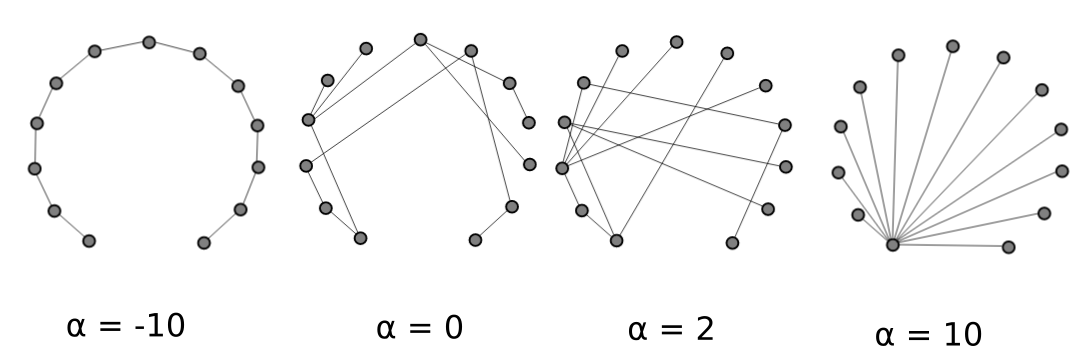
\includegraphics[width=1\linewidth]{chapter2/aging_nets.png}
	\caption[Aging model]{Aging model}
	\label{fig:aging}
\end{figure}

In the general ageing model, the non-linearity on the node degree is introduced, so this model has two tunable parameters $\alpha $ and $\beta$. The probability that a link is created between the new node and the existing node is defined as \cite{hajra2004}

\begin{equation}
\Pi_{i}(t)\sim k_{i}(t)^{\beta}\tau_{i}^{\alpha} 
\label{eq:1}
\end{equation}

As before, depending on model parameters network evolves into different structures:  
\begin{itemize}
	\item For example if we fix $\beta=1$ and $\alpha=0$ generated networks are scale-free; degree distribution is $P(k) \sim k^{-\gamma}$ with $\gamma=3$.
	\item In the case of nonlinear preferential attachment $\beta \neq 1$ and $\alpha=0$ scale-free properties disappear. 
	\item Scale-free property can be produced along the critical line $\beta(\alpha^{*})$ in the $\alpha-\beta$ phase diagram, see Figure \ref{fig:diagram}.
	
	\item For $\alpha>\alpha^{*}$ networks have \textbf{gel-like small world} behavior.
	
	\item For $\alpha<\alpha^{*}$ and near critical line $\beta(\alpha^{*})$ degree distribution has \textbf{stretched exponential} shape
	
\end{itemize}

\begin{figure}[h]
	\centering
	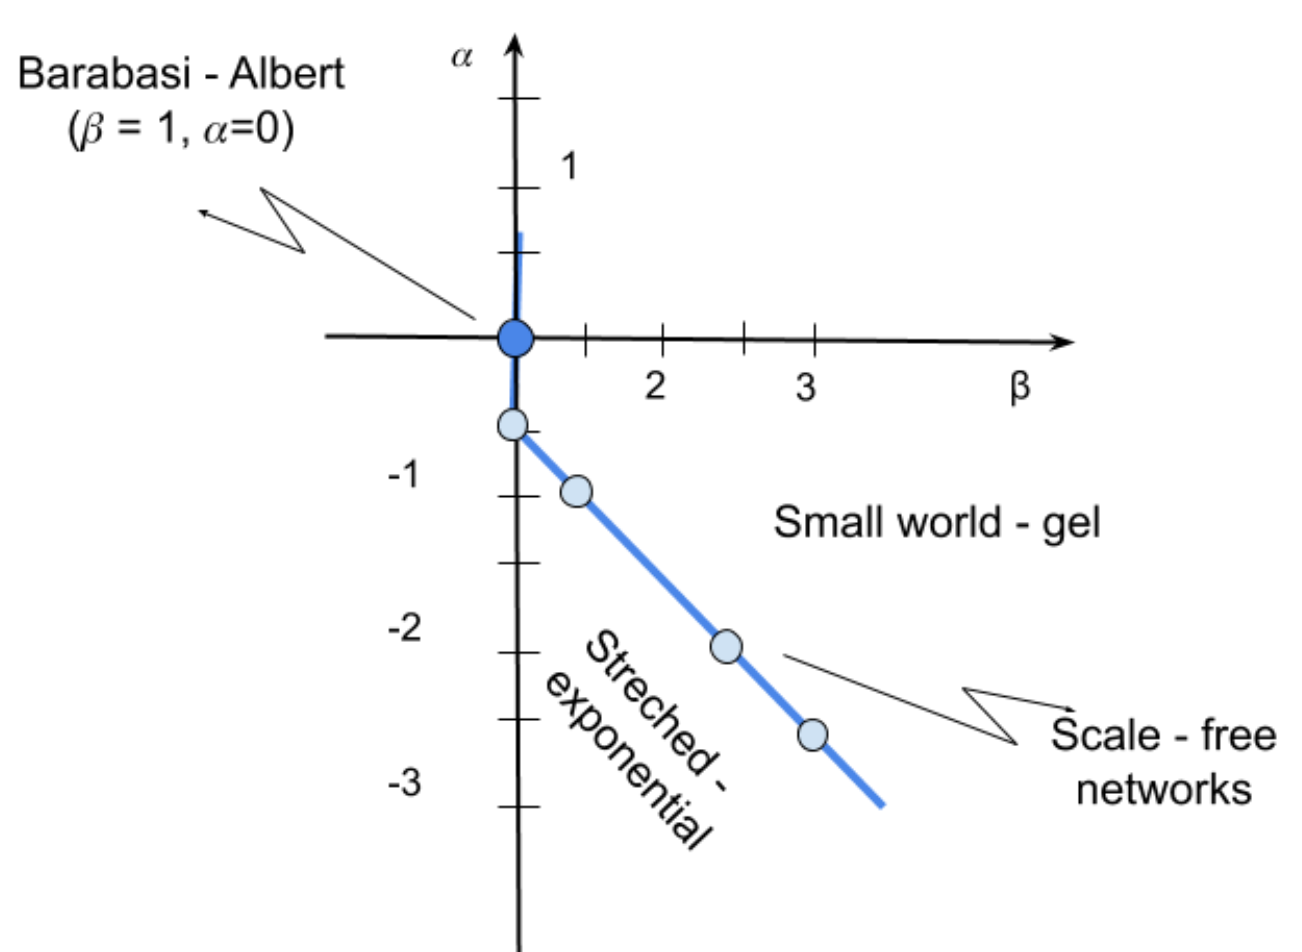
\includegraphics[width=0.6\linewidth]{chapter2/diagram.png}
	\caption[Phase diagram of aging network model]{Phase diagram of aging network model}
	\label{fig:diagram}
\end{figure}

\newpage

\section{The probability distributions}
%TODO mozda zameniti 2.3 i 2.4

The shape of degree distribution is important for getting the first insight into the characteristics of the complex network. When nodes are generated randomly, and any two nodes are linked with the same probability $p$,  we expect the binomial distribution. For larger networks it is Poisson distribution $P(k) = \frac{1}{k!}e^{-\langle k \rangle}\langle k \rangle^{k}$, where $\langle k \rangle = Np$. A different approach is to add one node and connect it randomly to the network at each time step. The obtained network then has the exponential degree distribution $P(k)=e^{-\lambda k}$. These are exponentially bounded distributions, meaning they decay exponentially or faster for the large values \cite{barabasi2016network}. 

On the other hand, heavy-tailed distributions decay slower than exponential, and the events for large values are rare but still possible. For example, in the preferential attachment model, degree distribution emerges to the power law \cite{barabasi2016network}. Also, many empirical data exhibit the heavy-tailed distribution. Even if they look like a power law, after statistical analysis, it may be concluded that the data deviate from the power law and could be equally good or even better fitted with some other distribution. Commonly used alternative distributions are lognormal distribution, stretched-exponential or power-law with an exponential cutoff. 

This section gives an overview of relevant distributions and methods for fitting data and testing the quality of the performed fit. 

%TODO Mozes da se ovde fokusiras na realne mreze vise neko na modelirane. Jer na kraju sve je krenulo od njih.

\subsection{The properties of distributions}

\textbf{Power-law distribution.} The power-law distribution \cite{mitzenmacher2004brief, newman2005power} is defined as 

\begin{equation}
p(k) = C k^{-\gamma}
\end{equation}
where parameter $\gamma$ is an exponent of the power-law distribution while the C is the normalizing constant. 

The distribution can take discrete and continuous values, defined for positive values $k>0$, so there is a lower bound to the power-law function $k_{min}$. For the discrete case $C=1/\zeta(\gamma, k_{min})$, while in the continuous case $C=(\gamma-1)k_{min}^{\gamma-1}$. 

The power-law distribution is called scale-free distribution. If we scale the value $k$ for the factor $2$, the ratio of $p(x)/p(2x)$ is constant and does not depend on the $k$ \cite{caldarelli2007scalefree}. We'll find that these criteria are not satisfied by any other distribution. 
\begin{equation}
\frac{p(k)}{p(2k)} = \frac{Ak^{-\gamma}}{A(2k)^{-\gamma}} = 2^{\gamma}
\end{equation}

The scale-free function is defined as $p(bx) = g(b)p(x)$. The solution of this equation is $p(x)=p(1)x^{-\gamma}$, where  $\gamma=-p(1)/p^{'}(1)$ leads us to the conclusion that if the function is self-similar, it has to be power-law.

\textbf{Lognormal distribution}. The variable $x$ has the lognormal distribution if the random variable $y=ln(x)$ is distributed as normal distribution \cite{limpert2001log}. 

\begin{equation}
f(y) = \frac{1}{2\pi\sigma}e^{-(y-\mu)^2/2\sigma^2}
\end{equation}
where $\mu$ is the mean, and $\sigma$ is the standard deviation. The density distribution of the lognormal distribution is defined as
\begin{equation}
f(x) = \frac{1}{x \sigma \sqrt{2\pi}}e^{-(log(x)-\mu)^2 /2\sigma^2} 
\end{equation}

The lognormal distribution has finite mean $e^{\mu+1/2\sigma^2}$, and the variance $e^{2\mu+\sigma^2}(e^{\sigma^2 -1})$.  \cite{mitzenmacher2004brief}. Despite the finite moments, the lognormal distribution can be similar to the power-law distribution. If the variance is large, then the probability function on the log-log plot appears linear for a large range of values. 

Using the \textbf{multiplicative processes}, we can generate the lognormal distribution \cite{caldarelli2007scalefree, mitzenmacher2004brief}. The lognormal distribution is generated by processes that economist Gibrat called the law of proportionate effect. If we start from the organism of size $S_0$. At each time step, the organism may grow or shrink according to the random variable $\epsilon$, 
\begin{equation}
S_t = \epsilon_t S_{t-1}
\end{equation}

When the system's state at time t is proportional to the state at the previous time step, we have the multiplicative process. The $\epsilon$ is a proportionality constant that can change over time. The current state depends only on the initial size $S_0$ and the $\epsilon$ variables.:
\begin{equation}
S_t = \epsilon_t S_{t-1} = \epsilon_t \epsilon_{t-1}... \epsilon_2 \epsilon_1 S_{0}
\end{equation}

If $\epsilon_t$ is drawn from the lognormal distribution, then $S_t$ also follows lognormal, as the product of lognormal distributions is again lognormal. Still, the $\epsilon$ distribution does not determine the distribution of the $S_t$. Taking the logarithm of the equation:
\begin{equation}
ln(S_t) = ln(S_0) + \sum_{i=0}^{t} ln(\epsilon_i)
\end{equation}

The sum of the logarithms of the $\epsilon_t$, according to the Central Limit Theorem (CLT), follows the normal distribution. The CLT states that the sum of identically distributed random variables with finite variance converges to the normal distribution. If $ln(S_t)$ is normally distributed, then $S_t$ follows the lognormal distribution.   

The multiplicative processes generate the lognormal distribution. Introducing a threshold in the multiplicative process leads to the power law. For example, in the Champernowne model \cite{caldarelli2007scalefree}, individuals are divided into classes according to their income. The minimum income is m. People between incomes m and $\gamma m$ are in the first class, and the second class are people with incomes between $\gamma m$ and $\gamma^2 m $. The individuals can change their class, so it is described as a multiplicative process, but with a threshold, as income can not be lower than m. If we fix $\gamma=2$, and consider that with probability $p_{i,i-1}=2/3$, the change is from higher to lower class. In contrast, with probability, $p_{i, i+1}=1/3$ individual goes to a higher class. In this process, the distribution of incomes emerges as the power-law distribution.

\textbf{Power law with exponential cutoff}. The density function has the following form 
\begin{equation}
p(k) = C k^{-\gamma}e^{-\lambda k}
\end{equation}
where $k>0$ and $\gamma>0$. This function combines the power-law, and exponential terms responsible for an exponentially bounded tail \cite{barabasi2016network}. Taking the logarithm $ln(p(k)) = lnC - \gamma lnk - \lambda k$, when $k<<1/\lambda$ the second term dominates, so distribution follows the power-law, with exponent $\gamma$. Otherwise, the $\lambda x$ term dominates, resulting in an exponential cutoff for high values. 

\textbf{Streched exponential} The stretched exponential distribution is defined as:
\begin{equation}
p(k) = c k^{\beta - 1}e^{-(\lambda k)^{\beta}}
\end{equation}
the parameter $\beta$ is stretching exponent determining the properties of the function $p(k)$ \cite{barabasi2016network}. For $\beta=1$, the function is exponential. For $\beta<1$, it is hard to distinguish the distribution from the power law. We have a compressed exponential function for $\beta>1$, so $k$ varies in the narrow range. 

%\subsection{Plotting the distributions}
%%TODO ovo ne treba da bude deo teze

%The first step in analyzing the empirical data is to create the frequency plot or histogram. Data are binned in equal intervals, and the number of data points within the interval are plotted. It is hard to determine whether the distribution is exponential or power law when plotting heavy-tailed distributions \cite{caldarelli2007scalefree}. If data are from power law distribution on the double logarithmic scale, they will look linear:
%\begin{equation}
%log p(k) = \gamma log(k) + c
%\end{equation}  
%On the log-log scale, we notice that noise in the tail of the distribution data exists. As the size of the bins is constant, the bins' density for large values also becomes large. To avoid the fluctuations in the tail, we can use logarithmic binning \cite{barabasi2014network, caldarelli2007scalefree, nair2022fundamentals}. The noise is reduced by dividing the $x$ axis into $n$ bins $b_n = c^n$, so the following bin is wider than the previous one. For the base $c$, we can choose any value $c>1$. Similarly, the binning can take the following form $b_n = k_0\exp{(cn)}$, where $k_0$ is the minimum data point, while the $c$ is the arbitrary base. All data points between values $[b_n, b_{n+1})$ are represented with one point $p(k_n) = N_n/b_n$, where $N_n$ is the number of nodes found in the bin $b_n$ and $k_n = \sum_i k_i / N_n$ is the average degree of the nodes in the bin $b_n$. By averaging over bins in the tail, noise in the tail of the distribution is reduced. Still, no matter how the bin size is chosen, the information about original data points is lost, especially in the distribution tail where bins are larger and include more samples. Figure \ref{fig:distributions} shows how different distributions look on linear (first column) and log-log scale (second column).

%\begin{figure}[!h]
%	\centering
%	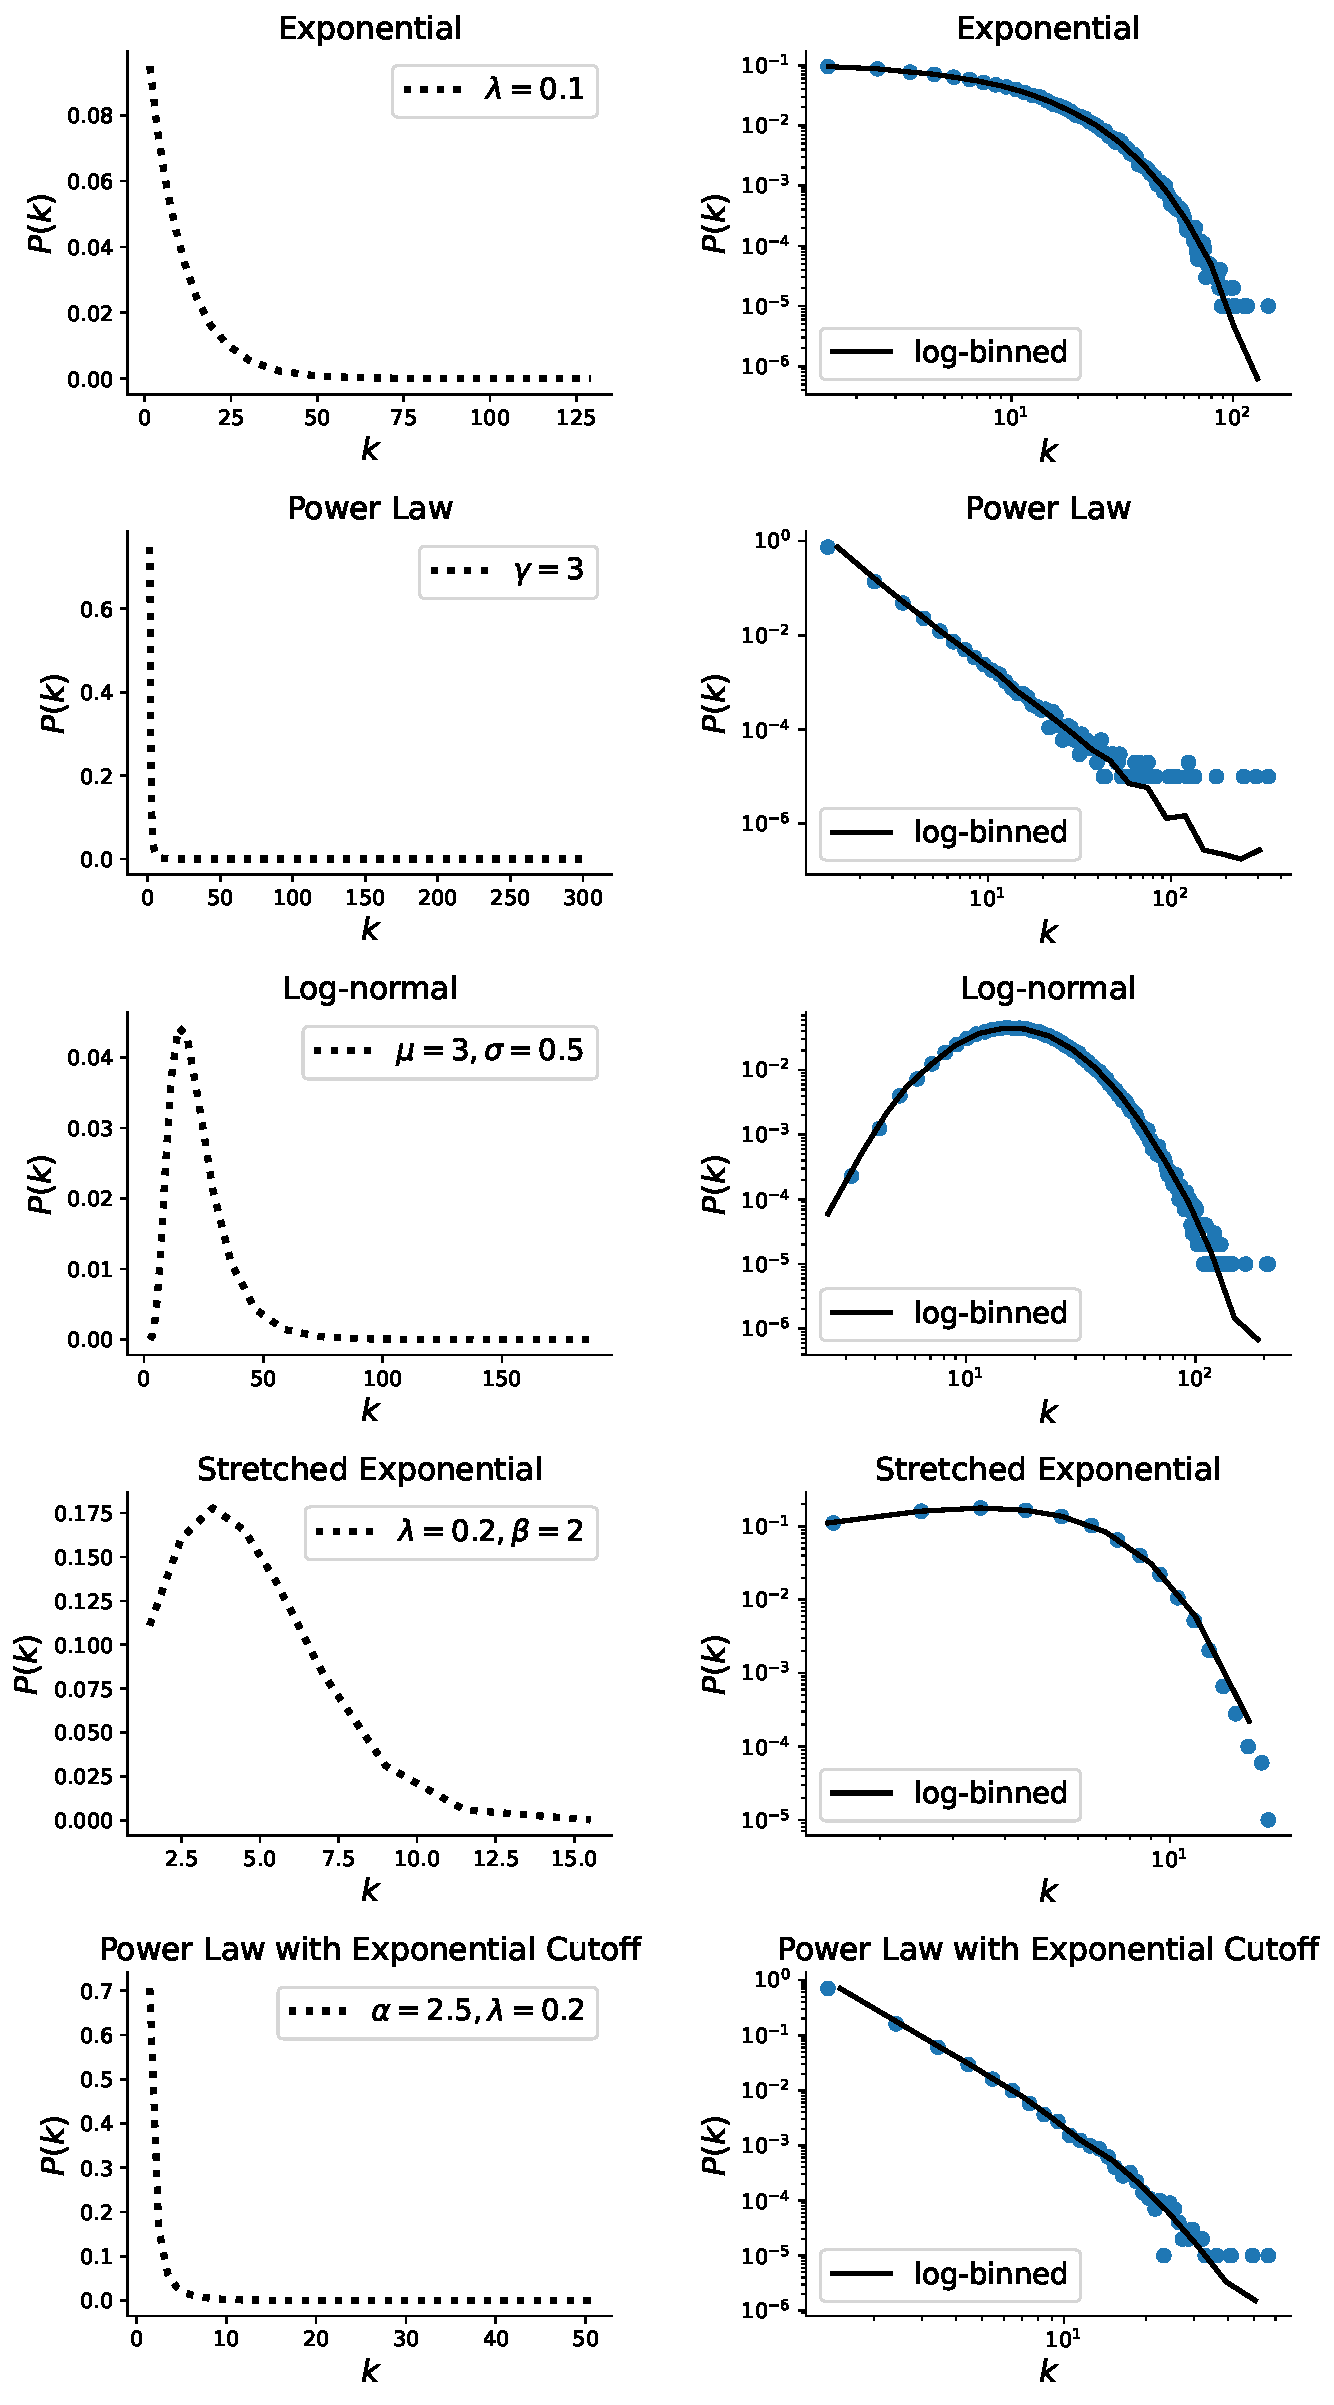
\includegraphics[width=0.75\textwidth]{chapter2/Distributions_plots.pdf}
%	\caption{Probability distributions on a linear and double logarithmic scale.}
%	\label{fig:distributions}
%\end{figure}

%Instead of plotting the probability distribution, it is possible to calculate the cumulative distribution, defined as $P(k) = \int_{k}^{\infty} p(k^{'}) dk^{'}$ for continuous function or as $P(k)=\sum_{k^{'}=1}^{k}p(k^{'})$ for the discrete function. For example, the CDF function for power law is also a power-law function but with exponent $\gamma -1$: $P(k)= k^{-(\gamma-1)}$. Note that for cumulative distribution, it is not necessary to use log-binning.

\subsection{Estimating the distribution parameters}

The maximum likelihood estimation(MLE) is a method where we consider that data comes from a particular distribution, so we want to maximize the likelihood of the data to find the distribution parameters. For a given set of i.i.d. observations $x_1, x_2, ...x_n$, sampled from the distribution $p(x)$, we can define the likelihood function  \cite{nair2022fundamentals}. The likelihood function tells us how likely it is to have the given data if the distribution parameters are $\theta$. 

\begin{equation}
L (\theta| x_1, ... x_n) = \prod_{i=1}^{i=n} p(x_i | \theta)
\end{equation}

The parameter that maximizes the likelihood function is $\theta_{max} \in arg max L(\theta| x_1,... x_n)$.

We can solve the equation and derive the expression for maximum likelihood parameters. The parameters can be obtained with numerical optimization for distributions where an analytical solution is unavailable. In practice is much easier to work with the logarithm of the likelihood function, $log(L) = \sum_{i=1}^{i=N} p(\theta| x_i)$, because then the product changes to summation. For the power-law distribution, the exponent is calculated as  
$\gamma = 1+n[\sum ln \frac{k_i}{k_{min}} ]^{-1}$. For a discrete distribution, the solution may be obtained by optimizing the log-likelihood function $log(L) = log\prod_{i=1}^{n} \frac{k_i^{-\gamma}}{\zeta(\gamma, k_{min})}$.

We can use the MLE \cite{clauset2009power} method to fit any distribution to the data. Even if obtained distribution looks like a power law, and some parameters are estimated, it does not have to be that data are truly from the power-law distribution. With the MLE method alone, it is impossible to distinguish between different distributions, and we do not know how accurate the obtained results are. To determine the quality of the fit, we need to use another statistical method called the \textbf{goodness-of-the-fit} test. The main idea is based on calculating the distance between distributions of empirical data and the model using Kolmogorov-Smirnov statistics. The Kolmogorov Smirnov statistics is the maximum distance between the CDF of the data and the fitted model, $D = max |S(x) - P(x)|$.

First, we fit empirical data to get model parameters and calculate the KS statistics of this fit \cite{clauset2009power}. Then, many synthetic data sets are generated with model-optimized model parameters. Then each synthetic data set is fitted, and KS statistics are obtained relative to its model. From there, we can calculate \textbf{p-value}, the fraction of times that KS-statistics in synthetic distributions is larger than in empirical data.  If $p-value<0.1$, we reject the hypothesis that this distribution describes the empirical data. Otherwise, the model can not be rejected. Failing to reject the hypothesis does not mean the model is a correct distribution for the data. Other distributions might fit the data equally good or even better. To have an accurate p-value, we need a large sample. For a small number of synthetic distributions, it is possible to have a high p-value, even if the distribution is the wrong model for the data. Finally, we need to be confident in obtained results. The same procedure can be repeated for different distributions. If the p-value for the power law is high, while for alternative distribution, it is low, we can conclude that the power law is a more probable fit. 

Another method, the \textbf{likelihood ratio test}, allows us to compare two distributions directly \cite{clauset2009power}. The distribution with a higher likelihood under empirical data is a better fit. We can calculate the likelihood ratio, or it is easier to obtain the likelihood ratio's logarithm because its sign determines which distribution is a better fit. For given two distributions $p_1(x)$and $p_2(x)$. 

The likelihoods are defined as $L_1=\prod_{i=1}^{n}p_1(x)$ and $L_2=\prod_{i=1}^{n}p_2(x)$, or the ratio of likelihoods as $R=\frac{L_1}{L_2} = \prod_{i=1}^{n} \frac{p_1(x)}{p_2(x)}$. Taking the logarithm, we obtain the log-likelihood ratio

\begin{equation}
\mathcal{R} = \sum_{i=1}^{n} \left[log p_1(x_i) - log p_2(x_i)\right]
\end{equation}

As data $x_i$ are independent, by central limit theorem, their sum $\mathcal{R}$ becomes normally distributed, with expected variance $\sigma^2$. We can approximate the variance as 

$$\sigma^2 = \frac{1}{n}\sum_{1}^{n}[(l_i - l_i) - (<l>^{(1)}- <l>^{(2)})]$$

When $R>0$, the first distribution is a better fit to the data, and then $R<0$, the other one should be chosen. When $R=0$, it is not possible to distinguish between two distributions. The sign of $R$ is not enough criteria to conclude which distribution is a better fit, and it is a random variable subject to statistical fluctuations. We need a log-likelihood ratio that is sufficiently positive or negative to ensure that its sign does not result from fluctuations.

If we are suspected that the expectation value of the log-likelihood ratio is zero, the observed sign of $\mathcal {} $ is simply the product of fluctuations and can not be trusted. The probability that the measured log-likelihood ratio has a magnitude as large or larger than the observed value R is given as

\begin{equation}
p = \frac{1}{\sqrt{2\pi n \sigma^2}} \int_{-\infty}^{-|\mathcal{R}|}e^{-x^2/2n\sigma^2}dx + \int_{|\mathcal{R}|}^{\infty}e^{-x^2/2n\sigma^2}dx
\end{equation}

Here we use the standard two-tail hypothesis test \cite{clauset2009power}, assuming that the null hypothesis is  $R= 0$. If the p-value is larger than a threshold, the R sign is unreliable, and the test does not favour any distribution. If p is small, $p<0.1$, then it is unlikely that the observed sign is obtained by chance, so we reject the null hypothesis that $R=0$. 
%\newpage

\section{Fractal analysis}

One of the approaches in studying complex systems is detecting the time series of selected variables \cite{kantelhardt2008fractal}. In complex systems, the periodic behaviour of time series is not limited to one or two characteristic frequencies. They extend over a broad spectrum and fluctuations on many time scales and broad distributions \cite{fan2012fractal, sidorov2018fractality}. In these cases, the system's dynamics are characterized by scaling laws, valid over a wide range of time scales or frequencies. When only one scaling exponent describes the system dynamics, the time series is monofractal.
On the other hand, we deal with multifractal time series. Rescaling time $t$ by a factor $a$ may require rescaling the time-series values $x(t)$ by a factor $a^H$; then, we have the self-similarity. The Hurst exponent, $H$, characterizes the type of self-affinity. 
$$x(t) = a^Hx(at)$$. 

\subsection{Long and Short-term correlations}
The time series are persistent, meaning that large values usually follow a large value \cite{kantelhardt2008fractal}. Considering the increments $\delta x_i = x_i - x_{i-1}$, of self-affine series $i = 1,.., N$, with N values measured equidistant in time, $\delta x_i$ can be either persistent, independent or anti-persistent. For the random walk with $H=0.5$, the increments are independent. For stationary data with constant mean and standard deviation, the auto-covariance function can determine the degree of persistence. 

\begin{equation}
C(s) = \langle \Delta x_i \Delta x_{i+s} \rangle = \frac{1}{N-s} \sum_{i=1}^{N-s}\Delta x_i \Delta x_{i+s}
\end{equation}


If the data are uncorrelated, the $C(s)=0$. Short-range correlations are described by $C(s)$ declining exponentially
$$C(s) = exp(-s/t_c)$$
such behaviour is typical for increments generated by an auto-regressive process 
$$ \Delta x_i = c\Delta x_{i-1} + \epsilon_i $$
with random uncorrelated offsets $\epsilon_i$ and $c = exp(-1/t_c)$.

For long-range correlations, $\int C(s)$ diverges in the limit for long series. In practice, this means that we can not define the characteristic time because it increases with N. Contrary to short-range correlations, the correlation function decline as power-law 
$$C(s) = s^{-\gamma}$$
Fourier filtering techniques can model this type of behaviour. Long-term correlated behaviour of $\Delta x_i$ leads to self-affine scaling behaviour characterized by Hurst exponent $H=1-\gamma/2$. 

A direct calculation of the $C(s)$ is complex due to present noise in the data and non-stationarity. Non-stationarities make the definition of $C(s)$ problematic because its average is not well defined. Also, $C(s)$ fluctuates around zero on large scales s, so it is impossible to obtain the correct correlation exponent $\gamma$. Instead of calculating $C(s)$, we can calculate the Hurst exponent $H$.

\subsection{Rescaled range analysis} 

Hurst proposed a method called the \textbf{rescaled range analysis} $R/S$, \cite{hurst1951long}. It begins with splitting the time series $x_i$ into non-overlapping segments $\nu$ of the size s, having $N_s = int(N/s)$ segments. Then is calculated the profile in each segment is. 

$$Y_\nu(j) = \sum_{i=1}^{j} (x_{\nu s +i} - \langle x_{\nu s + i } \rangle _s)$$

Substracting the averages, constant trends in the data are eliminated. The differences between minimum and maximum value and the standard deviation in each segment are calculated as $R_{\nu}(s) = max Y_\nu(j) - min Y_{\nu}(j)$, $S_{\nu}(s) = \sqrt{\frac{1}{s}\sum Y^2_{\nu}(j)}$

Finally, the rescaled range is averaged over all segments to obtain the fluctuation function F(s).

$$F_{RS}(s) = \frac{1}{N_s}\sum \frac{R_{\nu}(s)}{S_{\nu}(s)} \sim s^H$$

, where the H is the Hurst exponent. Values $H<1/2$ indicate long-term anti-correlated data while $H>1/2$ long-term positively correlated data \cite{kantelhardt2008fractal}. 

\subsection{Fluctuation analysis}
%%TODO pozvati se na slike

The \textbf{fluctuation analysis} is based on the random walk theory \cite{kantelhardt2008fractal}. For given time series $\{x_i\}$ with length N, we first define the global profile in the form of cumulative sum, equation \ref{eq:cumsum}, where $\langle x\rangle $ represents the average of the time series. 

\begin{equation}
Y(j) = \sum_{i=0} ^j (x_i - \langle x\rangle), \quad j=1, ..., N
\label{eq:cumsum}
\end{equation}
Figure \ref{fig:hurst_signals} shows examples of multifractal, monofractal and white noise signal with their global profiles.

\begin{figure}[h]
	\centering
	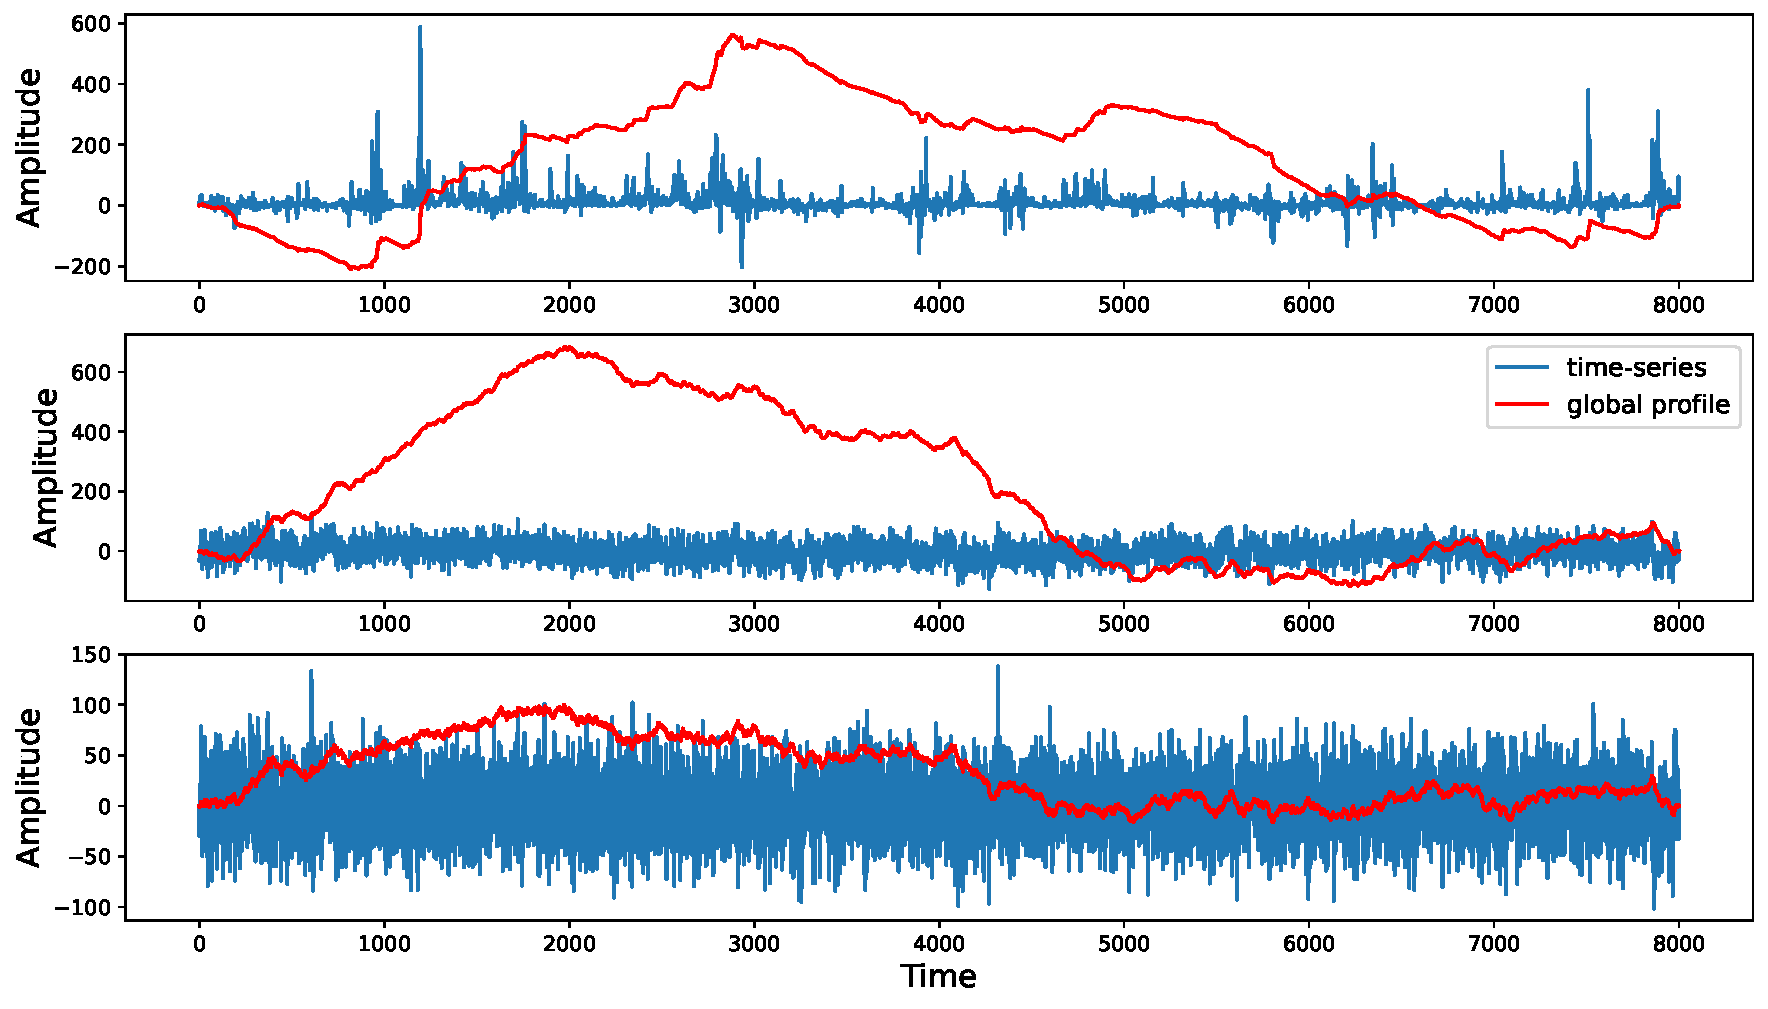
\includegraphics[width=0.8\textwidth]{chapter2/hurst_signals.pdf}
	\caption{Multifractal, monofractal and white noise signals.}
	\label{fig:hurst_signals}
\end{figure}

The profile of the signal Y is divided into $N_s = int (N/s)$ non-overlapping segments of length $s$. The last segment will be shorter if $N$ is not divisible with $s$. That is handled by doing the same division from the opposite side of the time series, giving us $2N_s$ segments. Then we calculate the fluctuations in each segment $F^2(\nu, s)$ and, finally, average overall subsequences, obtaining the mean fluctuation. From the scaling of the function, we can determine the Hurst exponent. 

\begin{equation}
F_2(s) = [\frac{1}{2N_s} \sum F^2(\nu,s)]^{1/2}  \sim s^H
\end{equation} 

Several methods are proposed for calculating the fluctuating function $F^2(\nu, s)$:
\begin{itemize}
	\item {The most straightforward way to calculate the fluctuations is to consider the difference in the values at the endpoints of each segment. It is the same as eliminating the linear trend from each segment.  
	$$ F^2(\nu, s) = [Y(\nu s) - Y((\nu +1)s)]^2$$ 
    Figure \ref{fig:hurst_detrending} shows the global profile of the multifractal signal, divided in segments of the length $s=1000$. On the top panel, each segment $s$ is approximated with linear function.
 }
	
	\item The trends present in the time series do not have to be linear \cite{hu2001effect}. The middle and bottom panel in Figure \ref{fig:hurst_detrending} show that the segments of the signal could be very well approximated with some higher order functions: quadratic or cubic. In general, using the detrended fluctuation analysis (DFA) we could remove the polynomial trend of the order $m$ \cite{kantelhardt2001detecting}.  
	% or any polynomial of order $m$. %When dealing with non-stationary time series, removing the polynomial trend within each segment is necessary by least-square fitting. 
	%The method where polynomial trend is removed is called detrended fluctuation analysis (DFA) .
	From each segment $\nu$, local trend $p^m_{\nu, s}$ - polynomial of order m - should be eliminated, and the variance $F^2(\nu, s)$ of a detrended signal is calculated as in equation:
	
	\begin{equation}
	F^2(\nu, s) = \frac{1}{s}\sum_{j=1}^s \left[Y(j) - p^m_{\nu, s}(j)\right]^2
	\label{eq:var}
	\end{equation}
\end{itemize}
\begin{figure}[h]
	\centering
	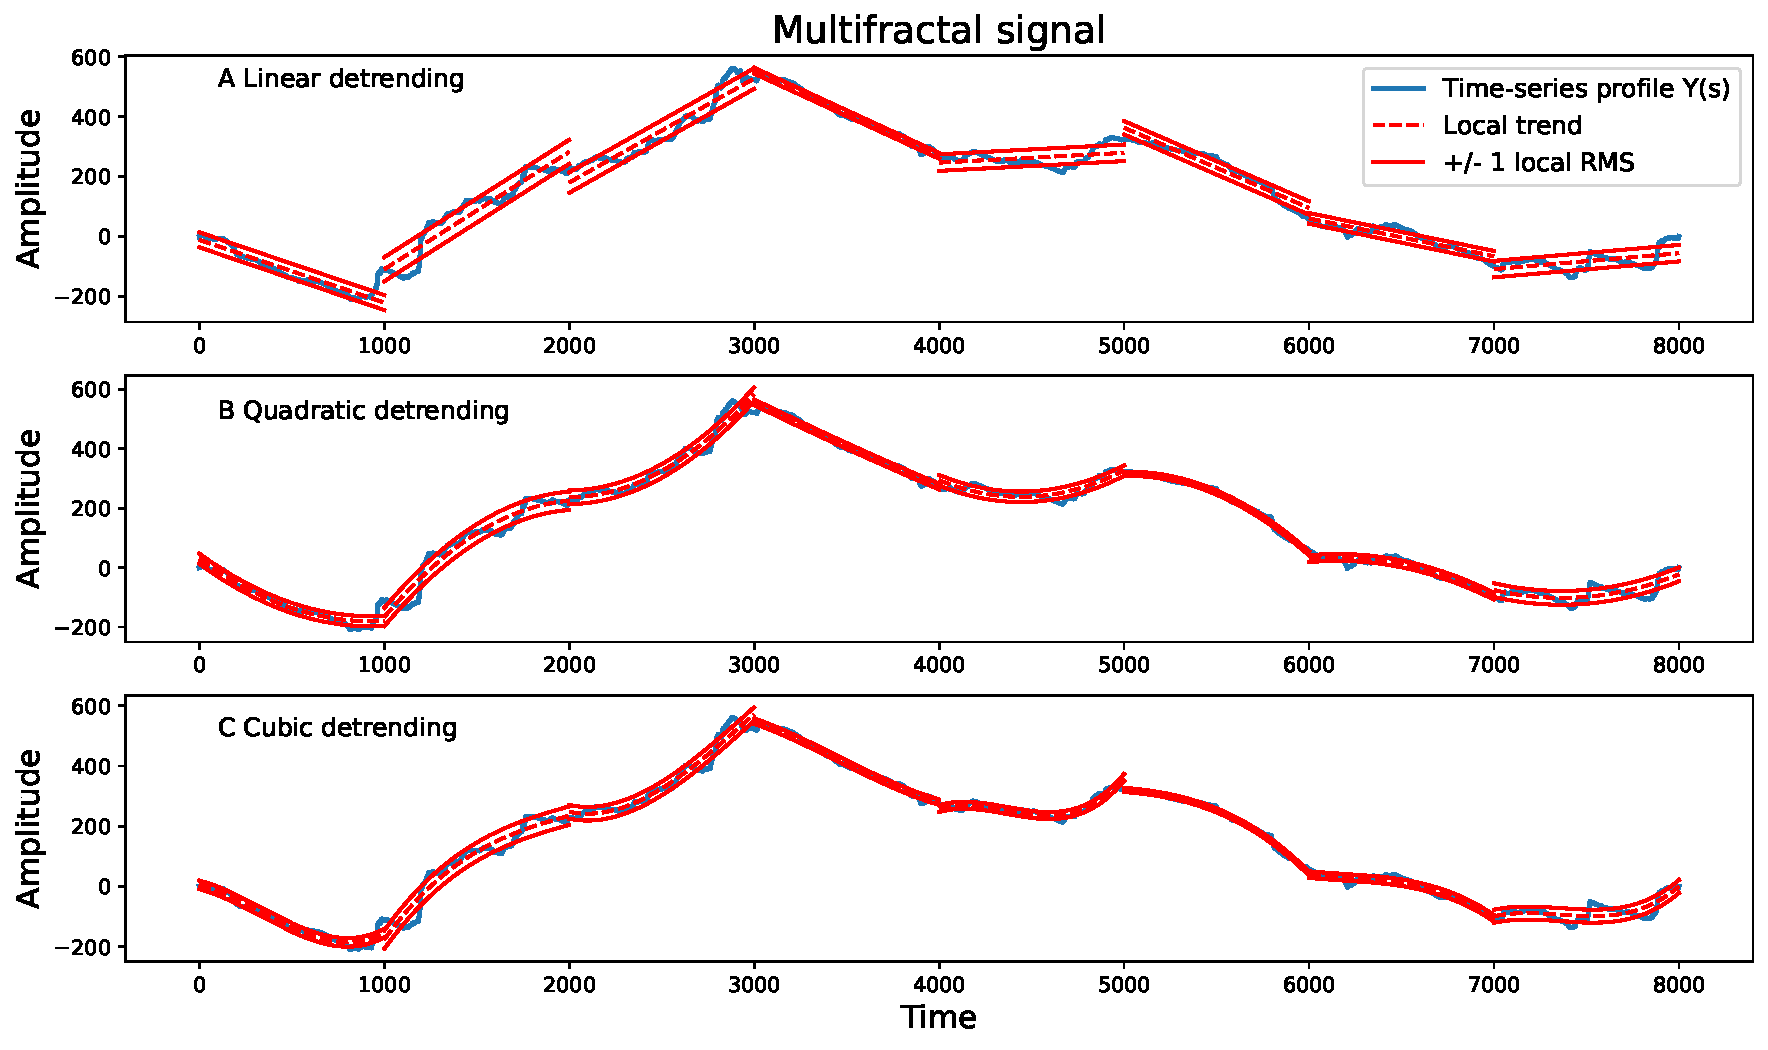
\includegraphics[width=0.8\textwidth]{chapter2/hurst_detrending.pdf}
	\caption{Detrending the signal for the segments of length $s=1000$.}
	\label{fig:hurst_detrending}
\end{figure}


\subsection{Multifractality of the signals}

The scaling behaviour in many data may be more complicated, and different scaling exponents can be found for many interwoven subsets of the time series, representing multifractal. The multifractality may come from the broad probability distribution of the time series values. In this case, the multifractal properties can not be destroyed with shuffling time series. The source of multifractality may be from different small and large fluctuations correlations. In this case, the probability density function of the values can be regular distribution with finite moments, and the corresponding shuffled series will exhibit non-multifractal scaling as correlations are destroyed with the shuffling procedure. When both kinds of multifractality are present, the shuffled time series will show weaker multifractality. 

The multifractal analysis will reveal higher-order correlations. Multifractal scaling can be observed if the scaling behaviour of small and large fluctuations is different. Multifractal detrended fluctuation analysis (MFDFA) is used \cite{kantelhardt2002, ihlen2012} to estimate multifractal Hurst exponent H(q). 

\begin{equation}
F_q(s) = \left\{\frac{1}{2N_s}\sum_{\nu}^{2N_s}\left[F^2(\nu, s)\right]^{\frac{q}{2}}\right\}^{\frac{1}{q}},  q \neq 0 \nonumber
\end{equation}

The MFDFA for $q=2$ is equivalent to the DFA method. The value of $H(0)$, which corresponds to the limit $H(q), q-0$, cannot be determined directly because the exponent diverges. Instead, the logarithmic averaging procedure has to be considered. 
\begin{equation}
F_0(s) = \exp \left\{\frac{1}{4N_s}\sum_{\nu}^{2N_s}ln \left[F^2(\nu, s)\right]\right\}, q=0
\end{equation}

The fluctuating function scales as power-law $F_q(s) \sim s^{H(q)}$ and the analysis of log-log plots $F_q(s)$ gives us an estimate of multifractal Hurst exponent $H(q)$, see Figure \ref{fig:hurst_mfdfa}

\begin{figure}[h]
	\centering
	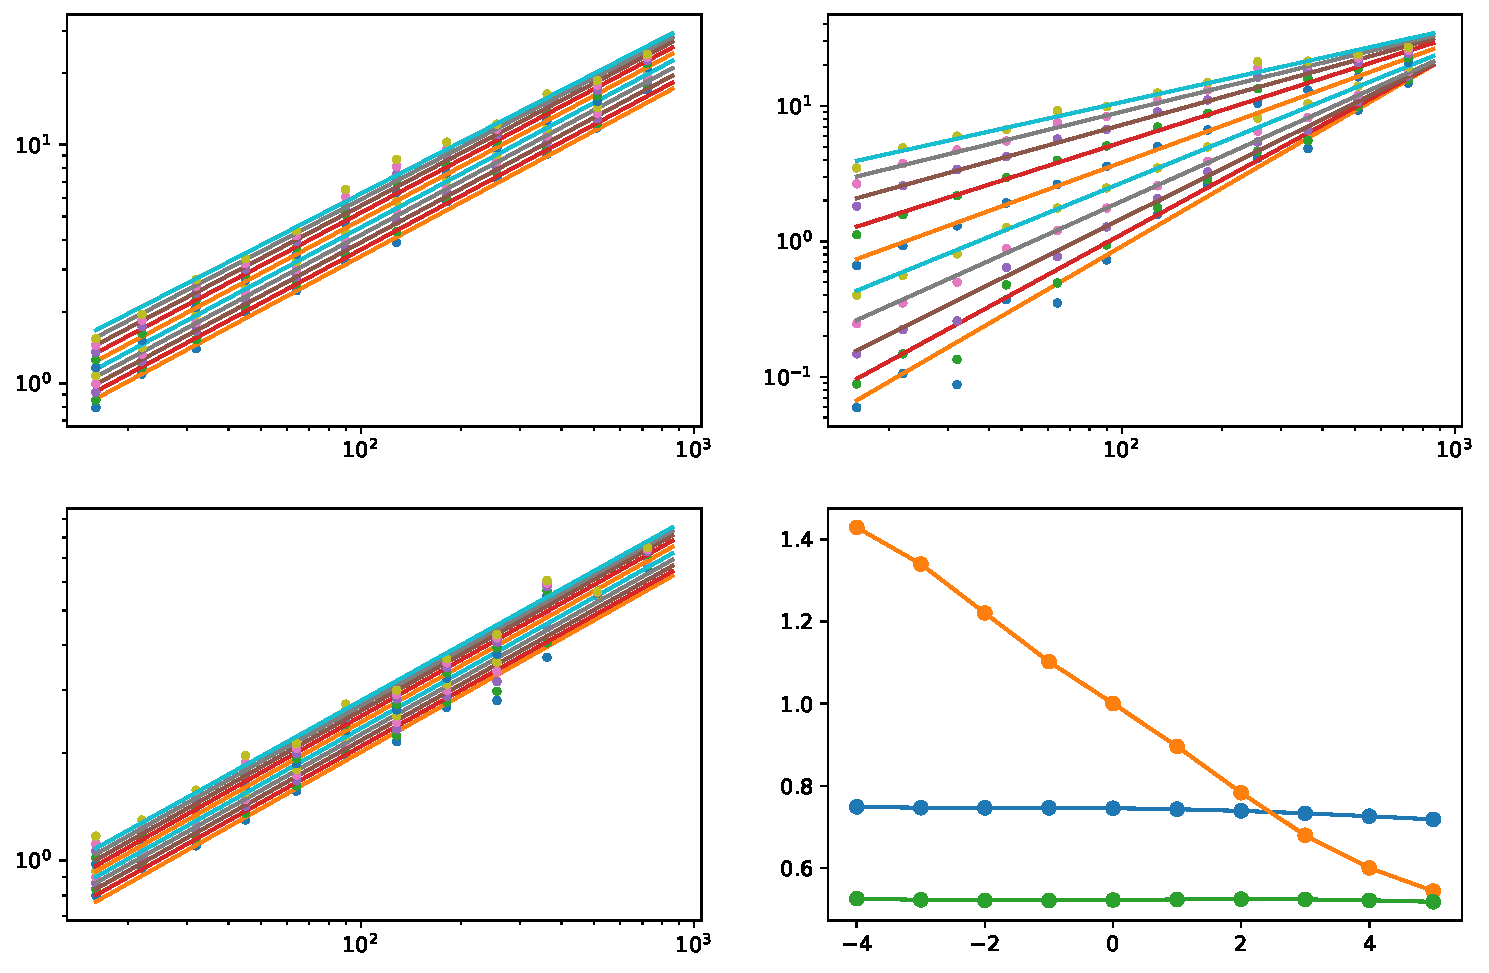
\includegraphics[width=0.8\textwidth]{chapter2/hurst_mfdfa.pdf}
	\caption[Fluctuating function and Hurst exponent.]{Dependence of the fluctuating functions on the scale for monofractal, multifractal and white noise signals, and the dependence of the Hurst exponent $H$ on the scale 1 $q$ for different types of signal (bottom right).}
	\label{fig:hurst_mfdfa}
\end{figure}

For the monofractal time series, H(q) is independent of q, meaning that scaling is identical for all segments, and averaging fluctuations gives identical scaling for all values of q. If small and large changes scale differently, h(q) will depend on q. Positive values of q, segments with large variance are dominant in the Fq(s), so positive q describes segments with large fluctuations. The negative values of q, H(q) describe the scaling of the segments with small fluctuations. 
%Also, large fluctuations are characterized by smaller scaling exponent. 

\section{Dynamical reputation model} \label{sec:met_dibrm}
%TODO Ok je da odredjivanje parametara bude u apednix-u ali to moras da kazes u samoj sekciji. Ja bih razmislila da moza odredjivanje parametara ne bude u apendixu nego ovde. I to je opcija.


Consider a system where each component has an activity pattern that could be mapped to the discrete signal, representing the moments when the event happened, such as the activity pattern when users are sending an email or communicating, sharing opinions and information within the community. Users' behaviour directly influences their position in the community, which is measured through reputation. The trust among users depends on the amount of interaction between them, which means the trust changes over time. The computational model needs to capture the dynamic property of the trust. Furthermore, the important property of the trust is that it is easier lost than gained; the frequency of interaction also matters. The trust between users who interact frequently should increase faster than between users who rarely interact. 

With Dynamic Interaction Based Reputation Model (DIBRM) \cite{melnikov2018toward}, we can quantify the user reputation $R_n$ after each interaction using equation \ref{eq:tn}, where $n$ is the number of interaction $n\in{1, N}$.
\begin{equation}\label{eq:tn}
R_{n}=R_{n-1} \beta^{\Delta_{n}} + I_{n}
\end{equation}

The first part of the equation considers the reputation value after the previous interaction $R_{n-1}$, weighted with coefficient $\beta^\Delta_{n}$. Depending on the frequency of the interaction, reputation will rise or decay. Parameter $\beta$ ranges from $0<\beta < 1$ is forgetting factor. The $\Delta_n$ measures time between two interactions $t_n$ and $t_{n-1}$: 
\begin{equation}\label{eq:deltan}
\Delta_{n}=\frac{t_{n}-t_{n-1}}{t_{a}}
\end{equation}
where $t_a$ is the characteristic time window of interaction. In the second part of the equation, $I_n$ is the reputation gained within each interaction. The basic value of each interaction is given as $I_{bn}$, and the parameter $\alpha$ is the weight of the cumulative part. 
\begin{equation}\label{eq:ibn}
I_n  = I_{b_{n}}(1 +  \alpha  (1-\frac{1}{A_n+1}))
\end{equation}

When $\Delta_{n}<1$, a user is frequently active, meaning that the time between two interactions is less than the characteristic time window. The number of sequential activities $A_n$ increases by 1. On the other hand, when $\Delta_n>1$ is large, the reputation decays, while the number of activities resets to $A_n=1$. 



\begin{figure}[h]
	\centering
	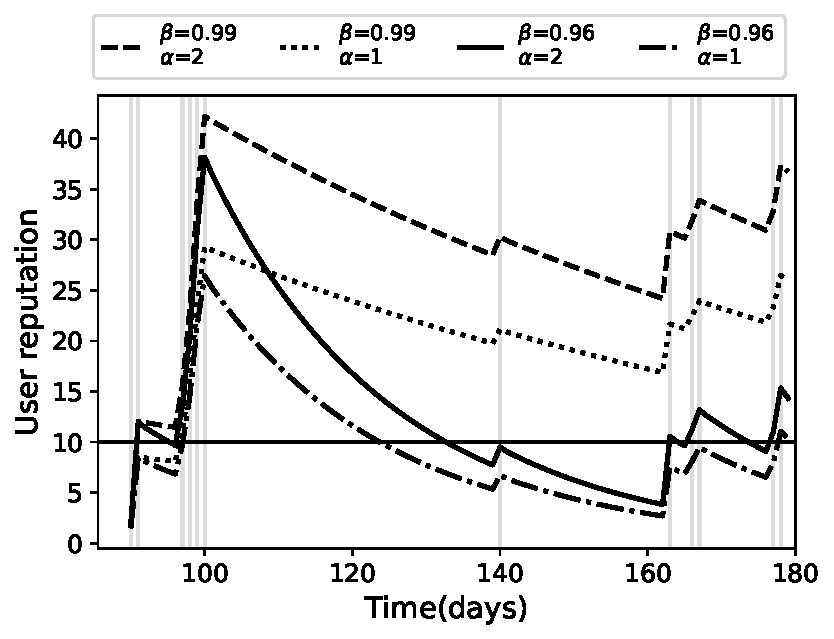
\includegraphics[width=0.45\textwidth]{chapter2/DIBRM.pdf}
	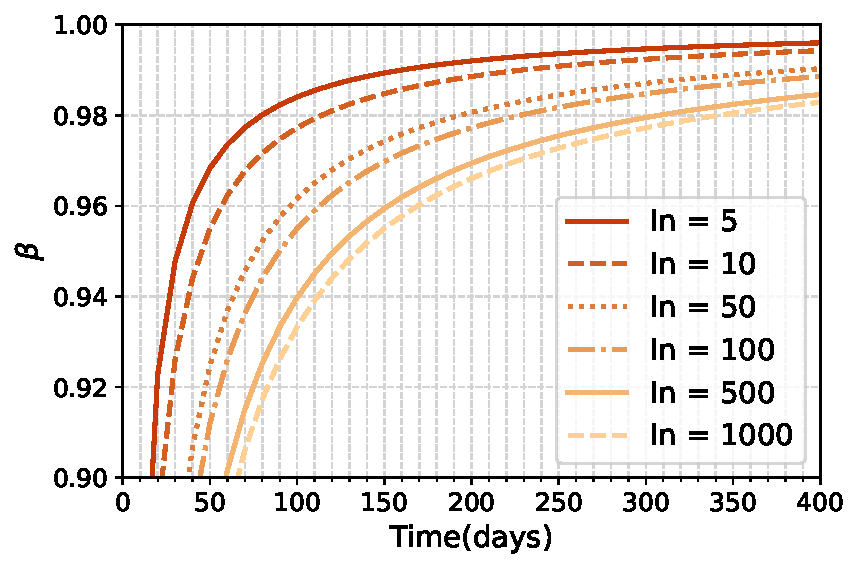
\includegraphics[width=0.45\textwidth]{chapter2/DIBRM_decay.pdf}
	\caption{User reputation.}
	\label{fig:reputation}
\end{figure}  

For example, if we set the characteristic window size and basic value of interaction to $t_a=1 day$, $I_{bn}=1$, we can analyze the influence of the parameters $\alpha$ and $\beta$ on the user reputation. Lower $\alpha$ and $\beta$ values lead to faster reputation decline, as shown in Figure \ref{fig:reputation} - left panel. With lower $\beta$, the reputation may quickly drop close to the reputation threshold, under which we don't consider the user as active. In contrast, with larger values of $\beta$, reputation stays high even if a user is inactive for a larger period. The parameter $\alpha$ is the most important influence on burst behaviour, where larger $\alpha$ leads to higher reputation values. 

If a user is frequently active, we can record the reputation after each day. On the other hand, if $t_n-t_{n-1}>1 \text{day}$ we need to interpolate the reputation values for each day between two interactions, $t_{n-1}<t_d<t_{n}$. To do that, we consider that due to inactivity, reputation will only decay, so it could be calculated as $R_d = R_{n-1}\beta^{\Delta_d}$, where $\Delta_d=(t_{d}-t_{n-1})/t_a$. 

When a user becomes inactive, its reputation starts to decline, and when it drops below the reputation threshold user does not have any influence on the community. We can approximate the dependence of parameter $\beta$ and time $\delta t$ needed for reputation to reach this level as $\beta = (\frac{R_0}{R_i})^{\frac{t_a}{\delta t}}$. In the examples in Figure \ref{fig:reputation}, - right panel, the parameter $t_a=1\text{day}$, while we vary different starting reputation levels $I_n$.   
For $\beta$ values below $0.96$, the decay is fast, and within two to four months of inactivity, even high reputation values are
reduced below the threshold. On the other hand, with values of $\beta$, the decay process is more differentiated, and the high
reputation becomes harder to lose, surviving up to a year of inactivity. For $\beta$ equal to $0.96$, reputation with starting value $5$ needs around one month to decay below the threshold. For higher reputations, $500$ or $1000$, the decay period is around $5$ months. 

In this model, the user's reputation changes continuously through time, decreases when the user is inactive and grows with frequent and constant user contribution. The highest growth of a user's reputation is found through bursts of activity followed by a short period of inactivity. With model parameters, $I_{bn}, t_a, \alpha, \beta$, the dynamic of user reputation may be controlled and adapted to different communities. If the community has its reputation system, we can also fit the model parameters to mimic the actual reputation dynamic. 















